%% ----------------------------------------------------------------
%% report.tex
%% ---------------------------------------------------------------- 
\documentclass{ecsgdp}         % Use the GDP Report Style
\graphicspath{{../figures/}}   % Location of your graphics files
\usepackage[numbers]{natbib}            % Use Natbib style for the refs.
\usepackage{listings}
\usepackage[nonumberlist,toc]{glossaries}
\usepackage{tikz}
\usepackage{multicol,lscape}
\usepackage{longtable,array,hhline}
\usepackage{todonotes}
\usepackage{pgf-umlsd}
\usepackage{menukeys}
\usetikzlibrary{positioning}
\usetikzlibrary{arrows}
\usetikzlibrary{arrows,shadows}
\usepackage{pgfplots}
\usepackage{bbding}
\usepackage{pgfgantt}
\usepackage[explicit]{titlesec}
\usetikzlibrary{calc}
\usepackage{environ}
\usepackage{pdflscape}
\usepackage[titletoc]{appendix}

\newcolumntype{L}[1]{>{\raggedright\let\newline\\\arraybackslash\hspace{0pt}}p{#1\linewidth}}
\newcommand{\eoline}{\tabularnewline \hline}

\newcommand*\rot{\rotatebox{90}}

\DeclareFixedFont{\chapternumberfont}{T1}{ppl}{m}{n}{2.0in}

%Modified from http://tex.stackexchange.com/questions/99310/fancy-chapter-title-page-for-entire-document
\titleformat{\chapter}[display]
  {\Huge\bfseries\color{black}}%
  {}
  {-1.75in}%
  {%
	\parbox[b]{.5\linewidth}{\raggedright #1}%
	\parbox[b]{.5\linewidth}{\raggedleft \raisebox{0.8in}{{\large\bfseries\chaptertitlename}} \chapternumberfont\thechapter}%
  }
  [\vspace*{0.5in}]

\titleformat{name=\chapter,numberless}[display]
  {\Huge\bfseries\rmfamily\color{black}}
  {} 
  {-1in}
  {\parbox[b]{.65\linewidth}{#1}}
  []


\usepackage{enumitem}
\usepackage[nameinlink]{cleveref}
\newlist{requirement}{enumerate}{1}
\crefname{requirementi}{Requirement}{Requirements} 

% Defines the language JavaScript for lstlistings
% Taken from http://tex.stackexchange.com/a/156326

\usepackage{color}
\definecolor{lightgray}{rgb}{.9,.9,.9}
\definecolor{darkgray}{rgb}{.4,.4,.4}
\definecolor{purple}{rgb}{0.65, 0.12, 0.82}
\lstdefinelanguage{JavaScript}{
  keywords={break, case, catch, continue, debugger, default, delete, do, else, false, finally, for, function, if, in, instanceof, new, null, return, switch, this, throw, true, try, typeof, var, void, while, with},
  morecomment=[l]{//},
  morecomment=[s]{/*}{*/},
  morestring=[b]',
  morestring=[b]",
  ndkeywords={class, export, boolean, throw, implements, import, this},
  keywordstyle=\color{blue}\bfseries,
  ndkeywordstyle=\color{darkgray}\bfseries,
  identifierstyle=\color{black},
  commentstyle=\color{purple}\ttfamily,
  stringstyle=\color{red}\ttfamily,
  sensitive=true
}

\lstset{
   language=JavaScript,
   backgroundcolor=\color{lightgray},
   extendedchars=true,
   basicstyle=\footnotesize\ttfamily,
   showstringspaces=false,
   showspaces=false,
   numbers=left,
   xleftmargin=20pt,
   numberstyle=\footnotesize,
   numbersep=9pt,
   tabsize=2,
   breaklines=true,
   showtabs=false,
   captionpos=b
}

% Defines a `datastore' shape for use in DFDs.  This inherits from a
% rectangle and only draws two horizontal lines.
\makeatletter
\pgfdeclareshape{datastore}{
  \inheritsavedanchors[from=rectangle]
  \inheritanchorborder[from=rectangle]
  \inheritanchor[from=rectangle]{center}
  \inheritanchor[from=rectangle]{base}
  \inheritanchor[from=rectangle]{north}
  \inheritanchor[from=rectangle]{north east}
  \inheritanchor[from=rectangle]{east}
  \inheritanchor[from=rectangle]{south east}
  \inheritanchor[from=rectangle]{south}
  \inheritanchor[from=rectangle]{south west}
  \inheritanchor[from=rectangle]{west}
  \inheritanchor[from=rectangle]{north west}
  \backgroundpath{
    %  store lower right in xa/ya and upper right in xb/yb
    \southwest \pgf@xa=\pgf@x \pgf@ya=\pgf@y
    \northeast \pgf@xb=\pgf@x \pgf@yb=\pgf@y
    \pgfpathmoveto{\pgfpoint{\pgf@xa}{\pgf@ya}}
    \pgfpathlineto{\pgfpoint{\pgf@xb}{\pgf@ya}}
    \pgfpathmoveto{\pgfpoint{\pgf@xa}{\pgf@yb}}
    \pgfpathlineto{\pgfpoint{\pgf@xb}{\pgf@yb}}
 }
}
\makeatother

\hypersetup{colorlinks=true}   % Set to false for black/white printing
\input{Definitions}            % Include your abbreviations

\lefthyphenmin=62 %remove hypenation
\righthyphenmin=62
\sloppy %justify text (only needed as hypenation removed)
\setcounter{tocdepth}{2} %down to subsection shown in contents
\setcounter{secnumdepth}{2} %down to subsection numbered

\newcommand{\preamblequote}[2] {
	\\ \\\begin{center}
	 ``#1'' \\ - \small{#2}
	\end{center}
}

\NewEnviron{preamble}{
	\vspace*{\stretch{1}}
	\textbf{\textit{\large{\BODY}}}
	\vspace{\stretch{2}}
	\clearpage
	\glsresetall
}

\makeglossaries
\glossarystyle{list}
\newacronym[description={A defined interface that allows the access of features of a program or service}]{API}{API}{Application Programming Interface}
\newacronym[description={The definition file is used by vgQuestions plugin to create the overlaid quiz/poll}]{DF}{DF}{Definition File}
\newglossaryentry{vgQuestions}{text=vgQuestions,name=vgQuestions,description={A plugin to overlay quizzes and polls to videos},plural=vgQuestions}
\newacronym[description={Managed Learning Environment. The overall system used by an educational establishment to facilitate and manage learning}]{MLE}{MLE}{Managed Learning Environment}
\newacronym[description={Virtual Learning Environment. Component of a Managed Learning Environment responsible for the online interactions of students and tutors}]{VLE}{VLE}{Virtual Learning Environment}
\newglossaryentry{eAssessment}{text=eAssessment,name=eAssessment,description={The process of making, viewing and scoring assessments using a computer},plural=eAssessments}
\newacronym[description={Computer-Aided Assessment. \textit{see \gls{eAssessment}}}]{CAidA}{CAA}{Computer-Aided Assessment}
\newacronym[description={Computer Assisted Assessment. \textit{see \gls{eAssessment}}}]{CAssA}{CAA}{Computer Assisted Assessment}
\newacronym[description={Computer Based Assessment. \textit{see \gls{eAssessment}}}]{CBA}{CBA}{Computer Based Assessment}
\newglossaryentry{authoring}{text={Authoring Tool}, name={Authoring Tool}, description={Tool responsible for creating the questions and assembling the test}, plural={Authoring Tools}}
\newglossaryentry{delivery}{text={Assessment Delivery System}, name={Assessment Delivery System}, description={Tool responsible for displaying and scoring the assessments}, plural={Assessment Delivery Systems}}
\newacronym[description={Question and Test Interoperability. Quiz interoperability standard by IMS Global. \url{http://www.imsglobal.org/question/\#version2.1}}]{QTI}{QTI}{Question and Test Interoperability}
\newacronym[description={User Agent Accessibility Guidelines}]{UAAG}{UAAG}{User Agent Accessibility Guidelines}
\newacronym[description={Web Content Accessibility Guidelines: \url{http://www.w3.org/TR/WCAG20/} (Accessed: 15 Jan 15)}]{WCAG}{WCAG}{Web Content Accessibility Guidelines}
\newacronym[description={Web Accessibility Initiative}]{WAI}{WAI}{Web Accessibility Initiative}
\newacronym[description={Massive Open On-line Course. A free study course available over the internet}]{MOOC}{MOOC}{Massive Open On-line Course}
\newacronym[description={Model-View-Controller. An architectural pattern used in creating user interfaces}]{MVC}{MVC}{Model-View-Controller}
\newglossaryentry{AngularJS}{text={AngularJS},name={AngularJS},description={A client side Model-View-Controller architectural pattern},plural={AngularJS}}
\newglossaryentry{Videogular}{text={Videogular},name={Videogular},description={HTML5 video player for \gls{AngularJS}},plural={Videogular}}
\newacronym[description={Representational state transfer. An architectural pattern focusing on simple interfaces, scalability, portability, reliability and modifiability of components}]{REST}{REST}{Representational state transfer}
\newacronym[description={Accessible Rich Internet Applications. A Web Accessibility Initiative technical specification from the World Wide Web Consortium (W3C) that specifies how to make web pages more accessible}]{ARIA}{ARIA}{Accessible Rich Internet Applications}
\newacronym[description={Document Object Model. A convention for accessing and updating objects in HTML and XML documents. It is cross-platform and language-independent}]{DOM}{DOM}{Document Object Model}
\newglossaryentry{webworker}{text={WebWorker},name={WebWorker},description={A sandboxed separate thread that runs
in the background of the webpage}, plural={WebWorkers}}
\newacronym[description={Cascading Style Sheets. Language used for specifying the styling of a document written in a markup language}]{CSS}{CSS}{Cascading Style Sheets}
\newacronym[description={HyperText Markup Language version 5. A language used to describe Web pages, which has come to refer to the combination of HTML5, \gls{CSS} and JavaScript}]{HTML5}{HTML5}{HyperText Markup Language version 5}

%% ----------------------------------------------------------------


\begin{document}
\frontmatter
\title      {Interactive Learning within Online Media:\\A Framework for Investigating Video eAssessment}
\authors    {
             {\href{mailto:cb15g11@soton.ac.uk}{Christopher Baines}}\\
             {\href{mailto:sb21g11@soton.ac.uk}{Samuel Bennett}}\\
             {\href{mailto:hc13g11@soton.ac.uk}{Harry Cutts}}\\
             {\href{mailto:cjh1e11@soton.ac.uk}{Christopher Hewett}}\\
             {\href{mailto:ml26g11@soton.ac.uk}{Maria Lynch}}
            }
\addresses  {\groupname\\\deptname\\\univname}
\date       {\today}
\subject    {}
\keywords   {}
\supervisor {Professor Mike Wald}
\examiner   {Dr. Gary B Wills}
\degree     {Master of Engineering Computer Science}
\maketitle
\begin{abstract}
This report details the creation of a framework for eAssessment within online videos.

Videos are often used as an educational tool within online learning systems, but limited information is known about the best way to include assessment within them.

Our framework allows for the direct inclusion of instant feedback quizzes within videos. It is hoped that in the future this framework will allow for a clear assessment of the viability of this learning model.
\end{abstract}
\tableofcontents

\listoffigures
\listoftables
\lstlistoflistings

\listoftodos
\newpage

\acknowledgements{The group would like to express their thanks to a number of people at the University who were instrumental in the success of this project.

Professor Mike Wald for both his exceptional supervision, and being a reasonable and communicative client.

Yunjia Li for his technical expertise on both Synote and software development in general.

Shameem Bajar for her help with gaining invaluable user feedback.

Dr Gary Wills for acting as an external source of help regarding the coursework.
}
\mainmatter
%% ----------------------------------------------------------------
%% ----------------------------------------------------------------
%% Introduction.tex
%% ---------------------------------------------------------------- 
\chapter{Introduction} 
\label{Chapter:Introduction}
\section{Problem} 
\label{Section:Problem}
Videos combined with quizzes and polls are often for educational purposes in many applications including \glspl{MOOC} and university lectures. For the authors of this resources this often involves splitting videos up into sections with a poll/quiz after each section to gauge understanding. Using this approach requires the author of the quizzes to have video editing skills in order to insert the quizzes. It would be useful if quizzes could be saved and included directly into the videos without the need to edit the videos. The new media created could be analysed to make discoveries about how best to present information to viewers so that they can take the most in. 

\section{Goals and Scope} 
\label{Section:Goals and Scope}
This project will be split into three main sections:
\begin{description}[%
  before={\setcounter{descriptcount}{0}},%
  ,font=\bfseries\stepcounter{descriptcount}\thedescriptcount~]
\item[Quiz Authoring Tool] \hfill \\
The authoring tool (designed with accessibility in mind) will allow users to:
\begin{itemize}
\item Specify sets of questions and polls to appear in the video
\item The time at which the question sets should appear
\item Actions that should be taken when the questions are answered (e.g. skip back to a certain point if the answer is incorrect)
\end{itemize}
The export will produce a JavaScript file (including a JSON schema) compatible with the video player that contains all of this information. 
\item[Overlaid Video Player] \hfill \\
A library will be implemented which allows quizzes and polls to be overlaid on Web videos, playable in the main browsers (Firefox, IE and Chrome) on different platforms (PC, Mac and Android). These videos could be any of the main video formats (MP4, WebM, OGG). The JavaScript files specifying the questions will be interpreted by the library and shown in the overlay. Accessibility considerations for the overlaid videos will be investigated.
\item[Video and Quiz Analytics] \hfill \\
Metrics of user behaviour will be recorded and methods of displaying these to the author will be explored.
\end{description}
%% ----------------------------------------------------------------
%% PreviousWork.tex
%% ---------------------------------------------------------------- 
\chapter{Previous Work} 
\label{Chapter:Previous Work}
\section{Academic Work} 
\label{Section:Academic Work}
A \gls{MLE} is the overall system used by an educational establishment to facilitate and manage learning. This will be comprised of several subsystems (as seen in \autoref{Figure: MLE}).

\begin{figure}[h]
	\centering 
		\includegraphics[scale=0.4]{../figures/MLE.png} 		
	\caption{\label{Figure: MLE} Components of an \gls{MLE} \citep{mle}} 	
\end{figure}

This project focuses on the Assessment system in the \gls{VLE}.

\subsection{eAssessment}
An \gls{eAssessment} (also known as \gls{CAidA}, \gls{CAssA}, \gls{CBA}) is the process of making, viewing and scoring assessments using a computer. In this report these processes will be carried out by several tools - the ``\gls{authoring}" will be responsible for creating the questions and assembling the test and the ``\gls{delivery}" will be responsible for displaying and scoring the assessments. These tools must be interoperable, meaning they must use data formats that are compatible with each other.

This project focuses on the use of quizzes and polls within videos as a means of assessment.

\subsubsection{Quiz Definition Standards}
\label{Subsubsection:Quiz Definition Standards}
In order to store and display the questions in an \gls{eAssessment}, a schema for the questions must be defined. The only formally defined standard found was IMS Global's \gls{qti} specification\footnote{\url{http://www.imsglobal.org/question/\#version2.1} Last Accessed: 24 Nov 14}. Some other quiz (wiki-like) definitions were found including Moodle's General Import Format Technology (GIFT)\footnote{\url{https://docs.moodle.org/28/en/GIFT_format} Last Accessed: 24 Nov 14} and Aiken formats\footnote{\url{https://docs.moodle.org/23/en/Aiken_format} Last Accessed: 24 Nov 14}.

GIFT is a question mark up by Moodle\footnote{\url{https://moodle.org} Last Accessed: 24 Nov 14}. It allows users to use a text editor to create questions in some simple formats. There is a strict compliance to specific syntax required and for complex questions it is no longer intuitive \citep{failQTI}. Aiken is another mark up that is designed to be more easily human-readable, again it has strict syntax that must be adhered to or the imports to Moodle would fail.

\gls{qti} is an interoperability standard for eAssessments. The specification overview \citep{qtiOverview} splits the \gls{eAssessment} system into five systems: authoring tool, item bank, test construction tool, assessment delivery system and learning system (see \autoref{Figure: QTI components}).

\begin{figure}[h]
	\centering 
		\includegraphics[scale=0.3]{../figures/componentsQTI.png} 		
	\caption{\label{Figure: QTI components} QTI components diagram \citep{qtiOverview}} 	
\end{figure}

In the \gls{qti} definition the authoring tool is used to create individual questions. However many systems combine this with the Item Bank and Test Construction Tool. For this report ``\gls{authoring}" refers to this combination and, as such, an authoring tool is used to create whole quizzes.

\cite{wikieassessment} state:
\begin{quote}
The major promise of QTI is that by introduction of common format developers can concentrate on developing innovative tools, whereas teachers can focus on defining new and groundbreaking methods of how to apply those tools in an online environment.
\end{quote}

It is a very complex specification with many ambiguous or optional elements. The complexity of the specification increases the likelihood for errors in the implementation as it opens up opportunities for developers to interpret the specification in different ways \citep{failQTI}. This means the intent of the original author may be lost.

\gls{qti} v2.1 was finalised in 2012 \citep{qtiOverview} but up to this point the standard was not widely used \citep{eps265979} as there were several fundamental flaws in the standard. When the v2.1 draft was withdrawn in 2009 Rib Abel (IMS GLC CEO) was quoted as saying (on v2.0) ``it’s deficiencies are well known and IMS does not recommend implementation of it [\dots] the only version of QTI that is fully endorsed by IMS GLC is v1.2.1"\footnote{\url{http://lists.ucles.org.uk/public/ims-qti/2009-March/001463.html}}. This standard gave definitions in natural language. These could often be long-winded and ambiguous, making the standard difficult to implement\citep{failQTI, Sclater2007}.

\gls{qti} v2.1 defines 18 types of interaction (question, answers and response patterns) \citep{qtiImplementation}:
\begin{multicols}{3}
\begin{enumerate}
\item Choice
\item Order
\item Associate
\item Match
\item Gap match
\item Inline choice
\item Text entry
\item Extended text
\item Hot text
\item Hotspot
\item Select point
\item Graphic order
\item Graphic associate
\item Graphic gap match
\item Position object
\item Slider
\item Drawing
\item Upload file
\end{enumerate}
\end{multicols}

In addition, assessment items can have template and/or adaptive behaviour giving 72 options for each item's type. 

Template items have variables in the questions and answers. These are set as the question is viewed. This allows similar questions to be defined using the same assessment item (e.g. changing the numbers in a maths problem).

Adaptive items are scored over a series of questions. Different questions are displayed based on the answer given for the previous question(s) in the sequence. This branching behaviour is defined by setting the \lstinline!adaptive! attribute to true. 

\subsubsection{Usage of Video in eAssessment}
\label{Subsubsection:Usage of Video in eAssessment}
Video is often used as a medium to convey educational material as it appeals to different learning styles. When video is streamed there is a lack of interactivity and user control \citep{eps267281}. To involve the user more, interactive elements must be added. \cite{eps267281} found that 75\% of users agreed or strongly agreed that interactive video had enhanced their learning experience but at the time of the paper there was no evidence of interactive video being used as a learning tool.

By adding polls and quizzes into videos immediate meaningful feedback can easily be given, a key feature of formative assessment \citep{eps265979}. Having the questions integrated into the video allows the appropriate sections to be automatically re-watched. 
\subsubsection{Accessibility and Usability}
\label{Subsubsection:Accessibility and Usability}
To allow interoperability between the \gls{eAssessment} systems the \gls{qti} specification involves both the model and the view of the data \citep{wikieassessment} making accessibility difficult to add in later. This means many systems that comply with the \gls{qti} specification are inaccessible. Moodle, for example, uses a video player to display content that is completely inaccessible to a user only using a keyboard\footnote{\url{https://tracker.moodle.org/browse/MDL-36081} Last Accessed: 24 Nov 14}.

\gls{eAssessment} systems require an authoring tool that is easily understood by people who do not have an in depth technical knowledge (e.g. teachers). Often authoring tools that implement the \gls{qti} standard are too technical for this \citep{wikieassessment}. These tools need to improve their accessibility and usability, keeping the time commitments for users reasonable \citep{eps271236, eps265979} or they will not be used.

There are many ways of conveying content in a video and none of the methods alone will generally convey the whole message. Most video searches stay on a whole resource level as there is a lack of semantic interlinking \citep{eps273063}. Annotation systems such as Synote\footnote{\url{http://synote.org/synote/} Last Accessed: 24 Nov 14} aim to make videos accessible by adding transcripts and other annotations to them. The videos being annotated may not be owned by the annotator.

\subsubsection{Analytics}
\label{Subsubsection:Analytics}



\newif\ifnote
\notefalse
\ifnote
In \cite{eps265979}:
R2Q2 (deprecated - replaced by QTI Engine)
Constructr - constructr.qtitools.org - proof-of-concept
Playr - playr.qtitools.org - deprecated - effectively our overlays
\fi

\section{Industrial Work} 
\label{Section:Industrial Work}

%% ----------------------------------------------------------------
%% OverallApproach.tex
%% ---------------------------------------------------------------- 
\chapter{Overall Approach} 
\label{Chapter:Overall Approach}
The overall project will use the AngularJS Framework. UIBootstrap will be used for all user interfaces
%% ----------------------------------------------------------------
%% ProjectManagement.tex
%% ---------------------------------------------------------------- 
\chapter{Project Management} \label{Chapter: Project Management}
This project was run using a SCRUM project management approach. This involved weekly SCRUM meetings where the issues in the backlog were discussed. They were prioritised and given a point value which related to how much time and effort the issue would take to resolve. The highest priority issues were then assigned. Each person had a maximum capacity of points for each week. 
%SCRUM roles
%Burndown charts and other statistics

To ensure that all work was backed up and available to the entire group a GitHub organisation\footnote{\url{https://github.com/soton-ecs-2014-gdp-12/}} was used. Separate repositories for each area of the project are located here for ease of access. Using GitHub made it easier to interact with other open source projects.

The group used \url{http://www.waffle.io} to manage the issues backlog as this would interface directly with GitHub.
%% ----------------------------------------------------------------
%% VideoPlayer.tex
%% ---------------------------------------------------------------- 
\chapter{Video Player} 
\label{Chapter:Video Player}

\section{Accessibility} 
\label{Section:Accessibility}
Videogular has the option to display HTML controls for the video player, replacing the browser's built-in controls. However, when the project began there was no way for the user to access these controls without a mouse.The main problem was that the controls did not identify themselves as interactive elements, and so could not be 'focused' (selected with the tab key). This also prevented them from being picked up by a screen reader.

Some online video players allow the player as a whole to be focused, and then controlled with various keyboard shortcuts. The problem with this method is that accessibility aids, such as screen readers, will not have information on these controls, and so users of those technologies will have to be instructed. It is also not accessible to users of a clicker, who can only press one key and so require individually focusable controls.

Instead, the controls were made individually focusable by using semantic markup where possible, and ARIA attributes otherwise. When a control is in focus, a visual indicator is displayed to highlight it. Buttons can then be pressed using the space bar (\fref{Figure:Accessibility/Screenshots/Button}); the scrub bar can be moved using the left and right arrow keys (\fref{Figure:Accessibility/Screenshots/ScrubBar}); and the volume can be adjusted using the up and down arrow keys when the mute button is focused (\fref{Figure:Accessibility/Screenshots/Volume}).

\begin{figure}
	\begin{subfigure}[]{\textwidth}
		\includegraphics[width=\textwidth]{accessibility/button}
		\caption{The play button when focused. In this state, pressing the space bar plays or pauses the video.}
		\label{Figure:Accessibility/Screenshots/Button}
	\end{subfigure}
	\begin{subfigure}[]{\textwidth}
		\includegraphics[width=\textwidth]{accessibility/scrub-bar}
		\caption{The scrub bar when focused. In this state, pressing the left or right arrow keys skips backwards or forwards in the video.}
		\label{Figure:Accessibility/Screenshots/ScrubBar}
	\end{subfigure}
	\begin{subfigure}[]{\textwidth}
		\includegraphics[width=\textwidth]{accessibility/volume}
		\caption{The mute button and volume control when the mute button is focused. In this state, pressing the space bar toggles mute, and the up and down arrow keys change the volume.}
		\label{Figure:Accessibility/Screenshots/Volume}
	\end{subfigure}
	\caption{Screenshots of the accessibility improvements made to Videogular's HTML controls.}
	\label{Figure:Accessibility/Screenshots}
\end{figure}

This solution is not completely clicker-accessible, but could be made so by introducing buttons to skip forwards or backwards, and to raise or lower the volume. It is a significant improvement on the original state, as keyboard users can now use the player. The improvements were submitted to the Videogular project\footnote{\url{https://github.com/2fdevs/videogular/pull/108}}, and are now part of Videogular 0.6.1.

\section{Compatibility} 
\label{Section:Compatibility}

One of the main focuses of this part of the project was to make sure the application was compatible with a range of platforms, operating systems and devices. The first challenge was to ensure that the player and overlay displayed correctly at a variety of resolutions and screen/window sizes. 

Apple iPhones provided a problem as iOS forced the video to be played in fullscreen mode. This is a design choice and there is no way to play the video inline, directives to do this are ignored by the browser.

This meant that the video paused at the correct time but as the video is in the native player the overlay was not visible unless the player is quit. There is no way of notifying the user that this needs to be done. A possible solution involves telling the user to quit out of the video when it is paused so they may answer the question. However this is not very user friendly. iOS software on Apple tablets however does not have this limitation and the video will play inline correctly as the device is large enough.

Android phones correctly interpret the inline directive and will properly play this. This ensures that the overlay is correctly applied and usable. This has been the primary focus on testing on mobile devices as it represents a very large portion of the market.

The overlay which displays the questions that the user is asked appears above the video and obstructs the view of the video. Placing the overlay in the middle of the screen requires a large amount of CSS to correctly locate it on the screen for mobile and smaller sized devices. There are still some issues with the popup location on some mobile devices because the browser reports one screen size and uses another. Until these devices are compliant with the specification it is time consuming to write code to fix each individual case.

The best user experience with this application is using it on a desktop that has an updated browser. This will definitely work and display as intended. As the screen size of the device gets smaller the user experience is significantly reduced as the video and poll overlay will be much smaller than recommended. To support a number of browsers and operating systems a range of video formats are supplied to the videogular plugin so that the browser may pick one that can be played.
%% ----------------------------------------------------------------
%% VideogularQuestions.tex
%% ----------------------------------------------------------------

\chapter{Videogular Questions} \label{Chapter:VideogularQuestions}

\begin{preamble}
A videogular plugin was written to provide the core functionality. It allows for questions to be overlaid on top of the video and handles user interaction.

This plugin is called videogular-questions or \gls{vgQuestions} for short.

It provides a utility library which wraps the messaging passing interface making it easy to create content (used for the \gls{DF}).

\end{preamble}

\section{Introduction}

This plugin was one of the primary focusses of the project, an accessible system presenting the user with questions overlaid on a video. A number of features were explicitly requested by the client such as question types (\cref{Req:Question types}) and the ability to let users re-watch content easily if questions were answered incorrectly (\cref{Req:Jumping to content}).

\section{Design}

\begin{figure}[h]
\makebox[\textwidth][c]{
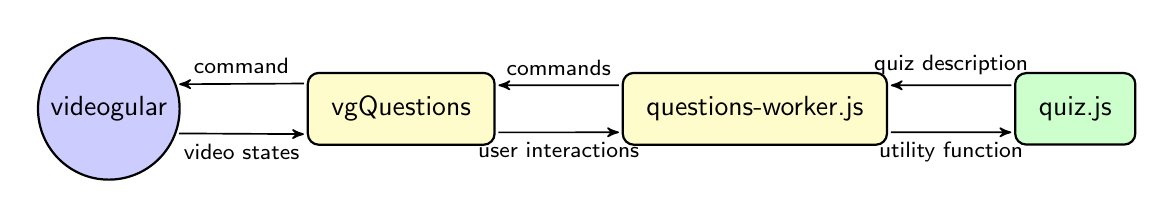
\begin{tikzpicture}[
  font=\sffamily,
  every matrix/.style={ampersand replacement=\&,column sep=1.6cm,row sep=1.6cm},
  source/.style={draw,thick,rounded corners,fill=yellow!20,inner sep=.3cm},
  vg-plugin/.style={draw,thick,rounded corners,fill=yellow!20,inner sep=.3cm},
  analytics-frontend/.style={draw,thick,rounded corners,fill=red!20,inner sep=.3cm},
  videogular/.style={draw,thick,circle,fill=blue!20},
  process/.style={draw,thick,circle,fill=blue!20},
  sink/.style={source,fill=green!20},
  datastore/.style={draw,very thick,shape=datastore,inner sep=.3cm},
  server/.style={source,fill=green!20},
  dots/.style={gray,scale=2},
  to/.style={->,>=stealth',shorten >=1pt,shorten <=1pt, semithick,font=\sffamily\footnotesize},
  between/.style={<->,>=stealth',shorten >=1pt,shorten <=1pt,semithick,font=\sffamily\footnotesize},
  every node/.style={align=center}]

  \matrix{
    \node[videogular] (videogular) {videogular}; \&
    \node[vg-plugin] (vg-questions) {vgQuestions}; \&
    \node[vg-plugin] (questions-worker) {questions-worker.js}; \&
    \node[server] (quiz) {quiz.js}; \\
  };

  \draw[to] (videogular.-20) --
      node[midway,below] {video states} (vg-questions.195);
  \draw[to] (vg-questions.-195) --
      node[midway,above] {command} (videogular.20);

  \draw[to] (vg-questions.-14) --
      node[midway,below] {user interactions} (questions-worker.190);
    \draw[to] (questions-worker.-190) --
      node[midway,above] {commands} (vg-questions.14);

  \draw[to] (questions-worker.-10) --
      node[midway,below] {utility function} (quiz.201); 
  \draw[to] (quiz.-201) --
      node[midway,above] {quiz description} (questions-worker.10);
\end{tikzpicture}
}
\caption{vgQuestions Architecture}
\label{Figure:vgquestions-architecture}

\end{figure}

The core of \gls{vgQuestions} is a \gls{DF} that is loaded in a \gls{webworker} that will talk to \gls{vgQuestions} as shown in \autoref{Figure:vgquestions-architecture}. This uses a well defined message passing interface to allow easy communication. As the \gls{DF} is provided by the user this makes the plugin exceptionally flexible. Many items of this can easily be changed to create a dynamic set of questions however most users will not interact with this directly.

The general use case is that the \gls{DF} will be generated through use of the authoring tool however the ability to manually create this file is open. This lets the user interface with the questions-worker.js library and configure the actions of the questions. The questions-worker.js library handles communication with vgQuestions, loading a JavaScript object that contains description of the quiz.

\section{Implementation}
The implementation of the questions overlay was split into three sections. The first was deciding how to represent the question sets internally. Next was how to represent the questions within the user interface. The final section was implementing the back end communication between the question representations and the video.

\subsection{Annotations}
\label{Section:Annotations}

One of the main issues to address early on was how to represent the quiz and poll questions. The \gls{QTI} specification was investigated, but was found to be complicated and incomplete \todo{What does incomplete mean here?} for the project needs. It was decided to design a new format for representing the data and logic that is used for a particular application of videogular-questions.

This new format separates the front end of the library (responsible for interacting with the \gls{DOM}), from the data and logic regarding the questions by means of a message passing interface. This is achieved in a rigorous way in the browser by means of a \gls{webworker}. This is a sandboxed separate thread that runs in the background of the webpage. They run independently of standard user-space scripts.  More can be found out about their use within this project in \autoref{Subsection:WebWorkers}

Using JavaScript, rather than a pure data representation (e.g. JSON or XML) allows you to include logic for the application to follow. This makes it extremely flexible and concise, and the isolation provided by the \gls{webworker} mitigates many security concerns with having an application that executes data given as input as code.

Every item in an annotation can have an action and condition function. The action function is called when a item finishes. The action function is given the state of the annotations, such that it can make decisions and then affect the state of the video accordingly. For example, in the above example, this is used to only have the ``skip back" question show, if the answer given to the previous question is incorrect.

The condition function is called to determine if the respective item will show. By default, when an annotation is shown, each item is shown in sequence. However, if an item has a condition function, this is evaluated, and the item only shown if the condition function returns \lstinline|true|. If the condition function returns \lstinline|false|, the item is skipped. This functionality is used in the above example to have the video skip back if the user wants it to.

An early decision was to define the difference between a poll and a quiz question. The decision made was that a poll is a type of quiz question that does not have a correct answer.

Initially basic question types (single choice, multiple choice and scale questions) were focused on. A variety of visualisations was implemented including check boxes, radio buttons and sliding scales. Validation was needed to ensure that the specified minimum and maximum limits were followed.

By having a standard \gls{DF} that uses JavaScript functions it was possible to write template functions that could be outputted from the authoring tool and read by the overlay correctly.

In reviewing the types of questions we would support we produced a class diagram (\autoref{Figure:questions_class_diagram}) to represent the type of data that the questions would have. Once the additional question types of textual and range were implemented this gave us conformance to \cref{Req:Question types}.

If the \lstinline|record_response| type was set to a \lstinline|true| value, the question would become a poll and report back the results to a server. If the \lstinline|correct_answer| attribute was set then the question would have a true value and would be shown to the user, if requested. This allows a user to possible have a poll type question that stores the data collected and also has a right answer. This provides maximum usability and therefore doesn't distinguish between a quiz or a poll in the underlying code.

Single question is a sub type of Multiple question where min and max (the minimum and maximum selected number of answers) is 1.

Similarly, the stars question is similar to the range question where the \lstinline|step value| is 1.

\autoref{code:questionworker} shows an example of the quiz definition file that could be used by the Videogular Questions plugin.

\begin{figure}
\centering
\includegraphics[width=12cm]{../figures/questions_class_diagram.png}
\caption{A class diagram representing what attributes each question type needs to detail}
\label{Figure:questions_class_diagram}
\end{figure}

\subsection{Front End - User Interface}

The appearance of the overlay depends on the question type to be shown. The layout of these different types was carefully considered for accessibility and ease of use. Mockups were made and user studies were done in collaboration with a third year project student.

A set of example \gls{CSS} files are supplied with the project that layout the questions according to the feedback received. Developers using any part of the project can use these styles as is, or modify/develop their own.

\subsection{Back End - WebWorkers}
\label{Subsection:WebWorkers}

\Glspl{webworker} give a good way of running (sandboxed) background scripts that are computationally intensive. They are a way of multithreading - allowing multiple scripts to run simultaneously, avoiding the problem of unresponsive pages due to long running scripts. This is done by using message passing.

For example, when an answer is submitted by the user this would sent a message to the \gls{webworker} containing the answer. The \gls{webworker} can then process this information without affecting the responsiveness of the page. Once the processing is complete the \gls{webworker} can send a message back to the page to tell it what to do next.

\begin{figure}

\centering

\begin{sequencediagram}
  \newthread[white]{c}{Front End}
  \newinst[4]{s}{WebWorker}

  \mess{s}{annotations}{c}

  \stepcounter{seqlevel}
  \begin{call}
    {c}{annotationStart}
    {s}{showQuestion}
  \end{call}

  \stepcounter{seqlevel}
  \begin{call}
    {c}{questionResult}
    {s}{showQuestion}
  \end{call}

  \stepcounter{seqlevel}
  \begin{call}
    {c}{questionResult}
    {s}{endAnnotation}
  \end{call}
\end{sequencediagram}
\caption{Sequence diagram showing interactions between the front end and webworker}
\label{Figure:sequence_diagram_frontend_webworker}

\end{figure}

\autoref{Figure:sequence_diagram_frontend_webworker} illustrates messages that could pass between the \gls{webworker}, and the front end when the above example is used. Initially, the worker sends an \lstinline|annotationStart| message which contains the times which annotations will occur.

When the first time point is reached, the front end sends a \lstinline|annotationStart| message to the worker containing the id of that annotation. The worker then replies with a \lstinline|showQuestion| message containing the contents of the first question. Note that here the functions are not sent to the front end and it is just the JSON representation of the question is sent.

When the user responds to the question, that response is sent to the worker in a \lstinline|questionResult| message. In this case the user responded incorrectly, therefore when the \gls{webworker} evaluated the condition on the second question it evaluated to \lstinline|false|. This meant that the worker replied with another \lstinline|showQuestion| message.

Once the user responds to the second question, the response is again sent to the \gls{webworker}. In this case, this was the final question in the annotation, so the worker responds with an \lstinline|endAnnotation| message.

\section{Conclusions}

An internal representation of the questions is given by the \gls{DF} that is used to display the questions to the user in the overlays. This allows all aspects of the questions presented to the user to be customised. This \gls{DF} can be manually written or it can be created by an authoring tool (\autoref{Chapter:Authoring Tool}).

We have used \gls{CSS} to keep the appearance of the questions consistent but this also allows a developer to quickly change how the questions are shown with little technical knowledge of the system helping to fulfil \cref{Req:Use of colour}.

\Glspl{webworker} are used to communicate with the front end to provide the necessary messages for the expected actions to occur. By abstracting this to another thread we have been able to utilise additional processing and ensure that the user has a good experience since the page is not likely to freeze due to the additional thread. In addition, separating the front end and back end and only communicating via a message passing system provides low coupling which will allows customising one without affecting the other.

\chapter{Authoring Tool} \label{Chapter: Authoring Tool}
%% ----------------------------------------------------------------
%% Analytics.tex
%% ---------------------------------------------------------------- 
\chapter{Analytics} \label{Chapter: Analytics}
%% ----------------------------------------------------------------
%% Testing.tex
%% ---------------------------------------------------------------- 
\chapter{Testing} \label{Chapter: Testing}

Talk about testing and how we will perform it.

Reference different plugins

Motivation for this.

{for section in sections: describe section}

\section{Videogular}

Comment on testing the video player

\section{Videogular Cuepoints}

Cuepoints, user stories, run through

\section{Videogular Heatmap}

Heatmap, user stories, run through

\section{Videogular Analytics}

Testing of sending events

\section{Authoring Tool}

Accessibility testing, List of objectives

Deliverable report had a basic list of actions to "test"

\section{Videogular Questions}

Example site as a test

regression tests using 

Client had reservations about UX testing due to toolkit style nature of the project. Shameem did so, results were interesting (possibly useful)

\section{Example poll server}

For the example poll server we had a small set of functions to test with a small number of possible inputs and a well defined set of responses. This is a therefore well suited to individual unit tests.

The flask library had a test client and recommended test skeleton\footnote{\url{http://flask.pocoo.org/docs/0.10/testing/}} which we made use of to run the unit tests. This used the unittest standard python library which meant it was easy to test with but also allowed calling of methods by simulating HTTP requests.

These tests are recommended to be run before committing new code to the repository and formed one part of the quality assurance testing. Any tests that failed were reviewed before committing and fixed if they were at fault. No code should have been committed to master branches that caused tests to fail. All code on the master branch was expected to pass these tests on checkout.

We split the testing into 6 areas to test the main components of the application.

\subsection{Cross-Origin Resource Sharing tests}

One of the main requirements by the customer \todo{Reference the requirement when they have been written} was that these units should be able to be accessed via REST calls. In addition the requirement stated that there should be no reliance that these servers are on the same host. To ensure that these REST calls will not fail we need to implement cross origin resource sharing headers as discussed in \autoref{Section:Modular Approach}.

This checks to ensure that the CORS header is correctly sent in the HTTP reply. If this is not set the web browser will likely reject the loading of the page and the application will fail.

In addition, it ensures that the response is the one expected and not an error state to ensure that the web application is also sending the correct content.

\subsection{Routing tests}

The routing tests are to ensure that the application correctly starts and is accessible.

If this fails to load up the testing URL which returns "Hello World!" then it is unlikely to be able to perform some of the more complex functions.

\subsection{Database Setup tests}

Before the application can be used it needs have its database set up. This is performed by accessing "/setup". This set of unit tests test setting up a database and ensure that if this URL is visited twice, it successfully detects that the database is already set up and does not recreate it. 

This is important to ensure that the database is set up correctly and that when setup is visited again data in the database is not lost.

\subsection{Voting tests}

These tests try a number of different ways to vote by sending a number of different formats of invalid and valid data to check if the application correctly deals with the data. All return codes and responses are checked to ensure no invalid vote is accepted or valid one rejected.

\subsection{Getting results tests}

A number of valid votes are constructed and then sent into the system. Then these are attempted to be retrieved. The returned values are checked to ensure that they have not been corrupted. This submits one and multiple votes to ensure that all votes are correctly collated and returned.

If the ability to vote does not work then this will fail as it relies on being able to put votes into the system.

\subsection{Load testing}

To be planned

\section{Example Analytics Server}

Load testing

\section{Conclusion}

Comment on the conclusions of the testing.


%% ----------------------------------------------------------------
%% FutureWork.tex
%% ---------------------------------------------------------------- 
\chapter{Future work} \label{Chapter: Future Work}

\begin{preamble}
This framework is very much just the beginning, there are a number of interesting improvements that can be made to enhance and extend the project. This chapter details a number of these potential improvements.
\end{preamble}

\section{Introduction}

During the project we have found a number of areas that could have been expanded. Some of these we have looked into but have not had time to further add to the project and others have been suggested as points of future work by our client. The most important items of future work have been detailed below.

\section{Integration with Synote}

The most important part of our project is ensuring that the work we have done is easily integrated into Synote.

Therefore during the process we have been in communication with the current developer of Synote to ensure that the work we are doing will be able to be used.

One key requirement was that the work we are doing should be able to stand alone and not require any additional Synote framework but that Synote should be able to communicate with these pieces of work easily (see \cref{Req:Standalone}).

To ensure this all, our services use an open standard to communicate using either \gls{REST} calls (\cref{Req:Server architecture}), with an associated documentation of each call and how it can be used, or protocols such as web sockets. These services can be run as small webservers which will allow Synote to communicate with them easily. In addition since these are standalone we have been able to pick the best language for the associated service. This has decreased the complexity of our services which should reduce the time needed to learn how the software works in order to continue our work.

The core of the project uses \gls{AngularJS} and the \gls{Videogular} player as this was recommended as the latest version of Synote will be written in Angular. All of the plugins were written for the \gls{Videogular} player and therefore will be able to be easily integrated into the primary Synote codebase. The plugins are the only part that will be integrated into Synote directly and therefore were best suited to be written in Angular. The other services will communicate with Synote and therefore did not need to be written in Angular.

\section{Additional Video Players}

Since our plugins are built upon the \gls{Videogular} system we have not been concerned with how the video is played. The base \gls{Videogular} system plays the common video formats.

To further expand our system we could look at fixing the \gls{Videogular} YouTube Plugin\footnote{\url{https://github.com/NamPNQ/bower-videogular-youtube}}. This would allow users to specify a youtube video to use for the quiz and removes the problems with getting all formats of video for all browsers.

This was not worked on due to the possible time requirement and was decided out of scope by the client. However some work was done looking into the changes required and it appeared to be possible to fix for the latest version.

\section{Video Encoding}

Video can be in many formats, there is software to perform the conversion, but to make this usable and transparent to the end user it would need to be integrated in to the video hosting/authoring tool.

The workflow would be as follows. User opens the authoring tool, and uploads a video. The server handing the video upload would then convert the video in to the set of required formats (assuming it is not in the single required format already).

This would be helpful to reduce the barrier to entry (\cref{Req:User interface}) as the user would not need to convert the video to the correct format.

\section{Mobile Interfaces}

Creating interfaces that work well with mobile interfaces is a difficult task and therefore we have only spent the time to ensure that our basic examples work on most mobile devices.

Further work would be concerned with getting the plugin to work on all devices as iPhones have shown to have significant issues with playing video and overlaying content (see \autoref{Section:Compatibility}).

\section{Second Screen}

A previous project \todo{cite} worked on the possibility of creating a second screening application that worked with Synote. This allowed you to have two views of Synote and display different data on a second screen. This screen would usually be a mobile device for audience members \todo{is this true?}.

If we had time to continue our work we would look into extending the plugin that we have developed to have a "second screen" option for users. This would allow users to turn their mobile device into a second screen for our popups to allow them to answer the questions on their device.

This would also allow a user to take advantage of additional lecture features such as subtitling. Another project is currently being ran to get in lecture subtitles and this could be a feature added as one of our plugins.

\section{Angular 2}

At the 2014 ng-europe conference during a talk about the future development of Angular details about the 2.0 release were given. It is slated for an early 2016 release, with Angular 1.x receiving bug fixes for anther 2 years.

Currently it seems that Angular 2.0 is a complete rewrite of the Angular ecosystem and is only related to Angular 1.x by name. Upon its release applications wishing to stay upto date will need to be rewritten from scratch. As this project is currently built around Videogular, it would first need to be updated and rewritten. This framework's main customer, Synote, is currently in development and as such is using Angular 1.x. 

As such there is potential future work for investigating Angular 2.0 upon its final release. At that time much more information regarding potential upgrade paths would exist.

\section{Accessibility}

\subsection{Cuepoints and Heatmap}
Currently the only way of getting information from the \gls{Videogular} Cuepoints is through the use of colour. \gls{Videogular} Heatmaps also has the option to include the frequency as text. Although the colours are customisable these plugins are not very accessible. An improvement that could be made in future is to have information available when the marked section is in focus (on hover and when it is playing) that gives the details used by the plugin. For example an area of a heat map could display the number of times the section has been viewed, and the start and end times of the section.

\section{Authoring Tool}
The authoring tool accessibility could be improved by adding support for accessibility features such as captions and transcripts. This would aid the improvement of the accessibility of the content when using it in the overlaid video player.

The elements used to create dropdowns and multiple select boxes could also be rewritten to allow the editing of colours in \gls{CSS}.

\section{Use of Graphs}
In our Example Analytics site graphs have been used as a representation but they have no textual alternative. In future, any graphs used should be made accessible to screen readers and users with cognitive impairments. 

\section{Conclusions}

The primary focus of our project towards future work has always been easing the integration into Synote. We have followed the requirements to ease integration (\cref{Req:Standalone}) to aid this.

As we have based our project on the Videogular player as a plugin, we have the ability to look into fixing the YouTube plugin. This will lower the barrier to entry (\cref{Req:User interface}) as users will not need to upload video and encode it correctly for different browsers. This was decided out of scope by the client. Another way of doing this would be automatically re-encoding the video on upload, which is a possible improvement too.

We did some research into mobile interfaces and found a number of problems with browser and differing phone behaviour and sizes. This is a very hard problem and therefore to focus on our original problem we did not look at doing this.

Previous work with second screening could be reviewed and re-implemented using out software but this would primarily rely on having the tools work on mobile devices (which are generally used for the second screening application).

Angular 2 does not look like it will present a problem as Angular 1 is likely to be around for a long time. Therefore the support of the application will not become problematic as deprecation of Angular 1 is not going to be soon.

Accessibility is a general topic that can be improved in all areas of our applications but much of these problems fall down to making the videos more accessible by adding captions and reducing the use of colours as the sole mean of conveying information. Keyboard accessibility (\cref{Req:Keyboard accessibility}) has been focussed on in terms of accessibility as this was one of the original requirements.

%% ----------------------------------------------------------------
%% Conclusions.tex
%% ---------------------------------------------------------------- 
\chapter{Conclusions} \label{Chapter: Conclusions}

\begin{preamble}
	The conclusions outlines the project and the degree of accomplishment focussing on client satisfaction as the primary measure of success.
	\preamblequote{It was a `Jump to Conclusions' mat. You see, it would be this mat that you would put on the floor; and would have different conclusions written on it that you could jump to!}{Richard Riehle as Tom Smykowski in Office Space (1999)}
\end{preamble}

%comments are from mark scheme

% ++ Points ++
%
% Video Player
%  - Several improvements made to Videogular (focuisng on accessibility)
%  - Compatibility with a range of devices was reviewed (problems with iOS)
%
% Videogular Questions
%  - The Definition File can be created manually or using the authoring tool
%  - The styling can be changed using CSS
%
% Authoring Tool
%  - Produces the Definition File
%  - Highly accessible
%  - The standalone nature of the plugins has allowed for there easy use in the
%  authoring tool
%  - The authoring tool allows previewing, making it easy to use
%
% Analytics
%  - Plugin allows the events to be sent over the network and recorded
%
% Testing
%  - Emphasis on integration tests and deliverable reports
%  - Example sites
%  - Unit testing for several repositories
%  - analytics front end as an integration test
%  - load testing
%
% Future work
%  - Primarily to aid integration with the future version of Synote
%  - Fixing the YouTube plugin
%  - Mobile devices need more testing, problems are not always solvable
%  - Second screening
%  - Angular 1 support is likely to continue, so this is not an issue. Also
%  Angular is not key to the project, as there are lots of components that could
%  be extracted and used without Angular
%  - Video accessibility (captions and colour)?

\section{Project Management}

Throughout the project, work was completed at a steady rate (\autoref{fig:tasksweek}) and work periods were distributed evenly over a 40 hour working week with some additional work at weekends and later at night (\autoref{fig:punch card}). The Gantt charts produced (\cref{App:Gantt Charts}) were used to track progress during meetings to ensure that client's priority deliverables had enough time.

The key to this project's success was the use of the agile software development
process. It allowed maximum reactivity and flexibility to ensure client
satisfaction. Regular meetings occurred between the developers and the client. These were
to keep the client apprised of the progress, and obtain the client's feedback on the
work done (\cref{App:Minutes of Meetings}). The development team also met regularly with additional meetings when necessary. During the start of the project, and some integration phases, it was beneficial to meet to work collaboratively. However, work was also done individually.


%Extensive review of related work and references; References relate both to academic and industrial work
%Excellent planning and progress, team worked independently, optimal use of team’s skills

%Justified evaluation of the strengths and weaknesses of the team, process, design, and results

\section{System Overview}

%Clear evidence of original thinking, considerable knowledge and understanding and ability to face considerable challenge

During the initial stages of the project, considerable effort was spent on fully comprehending the problem and investigating potential technical solutions. This resulted in an approach that, while being quite complicated, drew on a large number of tools and technologies. This provided the appropriate flexibility and functionality. 

The plugin (\gls{vgQuestions}) central to this project involved overlaying quizzes and polls onto videos. From the review of previous work it was found that instantaneous feedback is key to learning, therefore this was an important feature of the \gls{vgQuestions} plugin. Another important client requirement was that all plugins should be extensible. Using \gls{AngularJS} for the user interface of the \gls{vgQuestions} plugin, gives the required extensibility with the additional benefits of efficient reuse of code and high levels of customisability. 

In order for a dynamic set of questions to be displayed to the user, \glspl{webworker} (JavaScript sandboxed threads) have been utilised. This allowed for the use of a programmatic \gls{DF}, rather than using an exhaustive data format. This was a very different approach to using the \gls{QTI} definition standard; making accessibility considerations easier to implement without restricting the options available to authors.

The creation of the \gls{DF} is a non-trivial task. Thus, an authoring tool was produced to reduce the barrier to entry, enabling non-technical users to use the system. Accessibility considerations were a key factor in the development of the authoring tool to satisfy the client's requirements (\cref{Req:Keyboard accessibility} and \cref{Req:Use of colour}). 

In user generated sites that use the \gls{vgQuestions} plugin, there is the option to include analytics functionality provided by the \gls{Videogular} Analytics plugin. This enables future work researching the different ways users interact with eAssessment and learning systems to develop the next generation of interactive learning videos.

There have been a number of areas that are promising for further development in this system. The client is interested in additional plugins to handle additional video formats. The \gls{vgQuestions} abstraction supports different video formats without the need to modify any code in the plugin.

Further work towards accessibility (as outlined in \autoref{Section: Accessibility future work}) will increase the range of users able to use the system. A fully accessible system would allow new research that could improve eAssessment for people with disabilities.

\section{Summary}

During the project process, a number of important papers and research books have been reviewed to provide the necessary background in eAssessment (\autoref{Chapter:Previous Work}). Using the information gathered from both these academic and industrial works the team has produced an innovative  product that has fully satisfied the client.

Creating \gls{vgQuestions} and the associated tools in the framework has been a challenging project. It now allows users to go from the creation stage, through the publishing stage, and on to the analytics stage. Having met all goals the team looks forward to the client using the project within Synote, and hopefully seeing it used elsewhere online.

%Very challenging project, met all goals, ready to be used
%Publishable/patentable approach, thoroughly tested, evidence of client satisfaction


\newpage
\bibliographystyle{ecs}
\bibliography{ECS}

\newpage
\phantomsection
\markboth{GLOSSARY}{Glossary}
\printglossary

%TC:ignore
\appendix
\cleardoublepage
\addtocontents{toc}{\protect\setcounter{tocdepth}{1}}
\begin{appendices}
\chapter{Screenshots} \label{Chapter:Screenshots}

\begin{preamble}
	Screenshots of the software produced.
\end{preamble}

\section{videogular-questions-example}

\includegraphics[width=\textwidth]{screenshots/videogular-questions-example-poll-simple.png}

\includegraphics[width=\textwidth]{screenshots/videogular-questions-example-caesar-example.png}

\includegraphics[width=\textwidth]{screenshots/videogular-questions-example-question-single.png}

\includegraphics[width=\textwidth]{screenshots/videogular-questions-example-question-multiple.png}

\includegraphics[width=\textwidth]{screenshots/videogular-questions-example-question-stars.png}

\includegraphics[width=\textwidth]{screenshots/videogular-questions-example-question-text.png}

\includegraphics[width=\textwidth]{screenshots/videogular-questions-example-question-range.png}

\includegraphics[width=\textwidth]{screenshots/videogular-questions-example-poll-simple.png}

%prj mang
%% ----------------------------------------------------------------
%% AppendixProjectManagement.tex
%% ---------------------------------------------------------------- 
\chapter{Skills Audit Results} \label{App:Skills Audit Results}

\begin{preamble}
	An appendix detailing the skills audits that were performed.
	\preamblequote{Debugging is twice as hard as writing the code in the first place. Therefore, if you write the code as cleverly as possible, you are, by definition, not smart enough to debug it.}{Brian W. Kernighan}
\end{preamble}

\section{Skills Audit Matrices} 
\label{Section:Skills Audit Matrices}
A skills audit of the group members was performed and skills audit matrices was produced for all tasks relevant to the project.

Below we use acronyms for each group member in the tables. Each acronym relates to a below member of the group

\begin{itemize}
\item S - Samuel Bennett
\item H - Harry Cutts
\item CB - Christopher Baines
\item CH - Christopher Hewett
\item M - Maria Lynch
\end{itemize}

\subsection{Project Management} 
\begin{tabular}{ l || l | l | l | l | l || l}
  Task & S & H & CB & CH & M & Average \\ \hline
  Planning & 5  &  3  &  5  &  4  &  5  &  4.4 \\ 
  Progress tracking &  3  &  4  &  5  &  4  &  4  &  4.0 \\
  Time management &  5  &  4  &  5  &  4  &  4  &  4.4 \\
  Contingency planning &  4  &  4  &  5  &  5  &  5  &  4.6 \\
\end{tabular}

\subsection{Technical} 
\begin{tabular}{ l || l | l | l | l | l || l}
  Task & S & H & CB & CH & M & Average \\ \hline
  Technical Research &  4  &  4  &  4  &  5  &  5  &  4.4 \\
  Analysis &  5  &  4  &  4  &  5  &  5  &  4.6 \\
  Architecture Design &  3  &  5  &  4  &  5  &  4  &  4.2 \\
  API Design &  3  &  5  &  4  &  4  &  4  &  4.0 \\
  HCI / Interface Design &  4  &  4  &  4  &  5  &  5  &  4.4 \\
  Implementation \\
   - Client Side &  5  &  4  &  4  &  4  &  5  &  4.4 \\
   - Server Side &  4  &  5  &  5  &  5  &  4  &  4.6 \\
  Evaluation &  5  &  4  &  4  &  4  &  5  &  4.4 \\
\end{tabular}
%Implementation
%	Client Side
%		HTML
%		CSS
%		Javascript
%			AngualrJS
%	Server Side
%		Python
%			Flask
%		Javascript
%			Node

\subsection{Communication} 
\begin{tabular}{ l || l | l | l | l | l || l}
  Task & S & H & CB & CH & M & Average \\ \hline
  Technical Writing\\ 
   - Software Documentation &  4  &  5  &  4  &  5  &  5  &  4.6 \\
   - Report &  5  &  4  &  5  &  4  &  5  &  4.6 \\
  Academic Research &  5  &  4  &  4  &  5  &  5  &  4.6 \\
  Presentation &  5  &  5  &  4  &  4  &  4  &  4.4 \\
  Critical and comparative evaluation &  4  &  5  &  3  &  4  &  5  &  4.2 \\
  Reflection &  4  &  4  &  3  &  5  &  4  &  4.0 \\
\end{tabular}
\chapter{Coding Conventions} \label{App:Coding Conventions}

\begin{preamble}
	An appendix detailing the coding conventions and standards for the project.
	\preamblequote{How standards proliferate: \\ Situation: There are 14 competing standards \\ Researcher: 14?! Ridiculous! We need to develop one universal standard that covers everyone's use case! \\ Soon: \\ Situation: There are now 15 competing standards}{XKCD - web comic\footnote{XKCD Standards - \url{http://xkcd.com/927/}}}
\end{preamble}

\section{Introduction}

This appendix contains our coding conventions, from the GitHub repository
\footnote{\url{https://github.com/soton-ecs-2014-gdp-12/conventions}}.

\section{General}

File names should be in Unix form (lower-case, words separated by
hyphens, e.g. \texttt{a-directory/my-file.type}).

\section{CSS coding conventions}

Tabs should be used for indentation.

\subsection{Property ordering}

In general, properties further towards the top should affect layout,
while properties towards the bottom should affect appearance.

Specifically, the most common properties should be in this order:

\begin{lstlisting}
.class {
	position
	display

	flex /* etc. */

	top
	bottom
	left
	right
	z-index

	width  /* also min-, max- */
	height /* also min-, max- */

	padding
	border
	margin

	font /* etc. */
	text-align
	background /* etc. */
	color
}
\end{lstlisting}

\section{HTML coding conventions}

All full HTML pages should specify
\texttt{\textless{}!DOCTYPE html\textgreater{}}.

\subsection{Indentation}

Tabs should be used up to the indent level, with spaces for lining up
tags which break over multiple lines.

\subsection{Attributes}

Attribute values should be quoted.

The \texttt{id} attribute should always be first after the tag name,
followed by the \texttt{class} attribute. For meta tags, the
\texttt{name} should be specified first.

\subsection{Scripts}

Where possible, scripts should be imported at the end of the body. For
JavaScript files, the optional \texttt{type} attribute should be
omitted.

\section{Issue tracker usage guidelines}

If an issue doesn't seem to fit with any particular repository, file it
against the \texttt{videogular-questions} repository.

The issue type should be described with a label (one of bug,
enhancement, or investigate).

\subsection{waffle.io and Sprint management}

There is a waffle.io board
\footnote{\url{https://waffle.io/soton-ecs-2014-gdp-12/videogular-questions/}}
for tracking the Sprints.

Each Sprint will have a milestone on each repository, named ``Sprint '',
with the due date set to that of the Sprint Retrospective meeting. When
an issue is added to a Sprint, it should be added to that Sprint's
milestone.

\section{JavaScript coding
conventions}

Strict mode should be used (\texttt{'use strict';}). Semicolons should
never be omitted.

In object definitions, trailing commas should always be used. For
example:

\begin{lstlisting}[language=javascript]
obj = {
    foo: 'bar',
    baz: 'quux',
}
\end{lstlisting}

\subsection{Indentation}

Indentation should be done with tabs up to the indent level, and then
spaces for lining up multi-line statements. For example (where a
\texttt{\textgreater{}} is a tab and a \texttt{.} is a space):

\begin{lstlisting}[language=javascript]
function foo() {
>   if (bar === 4) {
>   >   baz("Some really ridiculously long string that should be "
>   >   ....+ "avoided, even mentioned in the coding conventions.");
>   }
}
\end{lstlisting}

This allows other developers to choose indent sizes without messing up
neatly lined-up parts.

\subsection{Naming}

Names should be camel case. The first letter should be lower-case,
except for class names or constructors:

\begin{lstlisting}[language=javascript]
LightBulb = (function() {
    function LightBulb() {
        // ...
    }

    return LightBulb;
})();

var numberOfEngineers = 5;
function changeLightBulb(bulb) {
    // ...
}
\end{lstlisting}

File names should still be in Unix form (e.g. \texttt{light-bulb.js}).
Unit test files should have the same name as the file which they test,
followed by \texttt{\_test} (e.g. \texttt{light-bulb\_test.js}).

\subsection{Types}

The section of JavaScript Garden on Types
\footnote{\url{https://bonsaiden.github.io/JavaScript-Garden/\#types}}
gives a number of guidelines (in the conclusion paragraphs) which should
be followed.

\subsection{JSHint}

JSHint directive comments should be kept to a minimum, with
configuration moved into the \texttt{.jshintrc} file where possible. If
file-specific configuration is necessary, it should go at the top of the
file (before \texttt{'use strict';}) unless:

\begin{itemize}
\item
  it is specific to a section of the file, or
\item
  it describes the changes made to the environment by a particular line
  of code, for example by the \texttt{importScripts} method in a Web
  Worker. In this case the directive should be on the next line,
  indented. For example:

\begin{lstlisting}[language=javascript]
importScripts("../../app/bower_components/videogular-questions/questions-worker.js");
    /* global loadAnnotations */
\end{lstlisting}
\end{itemize}

\subsection{AngularJS}

\subsubsection{Dependency injection}

When defining a directive, service, view, controller, etc., and
dynamically injecting dependencies, make sure to pass the parameter name
as a string into the array. For example:

\begin{lstlisting}[language=javascript]
angular.module("com.example.foobar", [])
    .directive(
    "ngFooBar",
    ["$window", "VG_STATES", function($window, VG_STATES) {
        ...
    }])
\end{lstlisting}

This stops minifiers from breaking the dependency information when they
rename parameters.

\section{LaTeX}

\subsection{TODOs}

For todo notes, use the \texttt{\textbackslash{}todo} command. For
example:

\begin{lstlisting}[language=tex]
\todo{Discuss farming in the Middle East.}
\end{lstlisting}

\subsection{References}

When making references, use \texttt{autoref}, like so:

\begin{lstlisting}[language=tex]
\autoref{my-label}
\end{lstlisting}

\subsection{Labelling scheme}

Figure labels should begin with \texttt{Figure:}, chapter labels with
\texttt{Chapter:}, and section labels with \texttt{Section:}.

\section{Python coding conventions}

PEP8 \footnote{\url{http://legacy.python.org/dev/peps/pep-0008/}} should be
followed.

\subsection{File names}

File names should be Python style, that is, words separated by
underscores (e.g. \texttt{voluminous\_octopus.py}).

When a virtual environment is used, it should be called \texttt{venv}.
Any dependencies should be defined in \texttt{requirements.txt}.

\chapter{Repositories} \label{Chapter:Repositories}
\section{Deliverables}

\subsection{videogular-questions}

\url{https://github.com/soton-ecs-2014-gdp-12/videogular-questions.git}

\subsubsection{Contributors}
\begin{itemize}
  \item Christopher Baines
  \item Christopher Hewett
  \item Harry Cutts
  \item Samuel Bennett
\end{itemize}

\subsection{videogular-analytics}

\url{https://github.com/soton-ecs-2014-gdp-12/videogular-analytics.git}

\subsubsection{Contributors}
\begin{itemize}
  \item Christopher Baines
  \item Christopher Hewett
  \item Harry Cutts
\end{itemize}

\subsection{videogular-cuepoints}

\url{https://github.com/soton-ecs-2014-gdp-12/videogular-cuepoints.git}

\subsubsection{Contributors}
\begin{itemize}
  \item Harry Cutts
\end{itemize}

\subsection{videogular-heatmap}

\url{https://github.com/soton-ecs-2014-gdp-12/videogular-heatmap.git}

\subsubsection{Contributors}
\begin{itemize}
  \item Christopher Baines
  \item Maria Lynch
\end{itemize}

\subsection{authoring-tool}

\url{https://github.com/soton-ecs-2014-gdp-12/authoring-tool.git}

\subsubsection{Contributors}
\begin{itemize}
  \item Christopher Baines
  \item Christopher Hewett
  \item Harry Cutts
  \item Maria Lynch
\end{itemize}

\section{Examples}

\subsection{example-poll-backend}

\url{https://github.com/soton-ecs-2014-gdp-12/example-poll-backend.git}

\subsubsection{Contributors}
\begin{itemize}
  \item Christopher Hewett
  \item Samuel Bennett
\end{itemize}

\subsection{example-analytics-backend}

\url{https://github.com/soton-ecs-2014-gdp-12/example-analytics-backend.git}

\subsubsection{Contributors}
\begin{itemize}
  \item Christopher Baines
  \item Christopher Hewett
  \item Harry Cutts
  \item Maria Lynch
\end{itemize}

\subsection{videogular-questions-example}

\url{https://github.com/soton-ecs-2014-gdp-12/videogular-questions-example.git}

\subsubsection{Contributors}
\begin{itemize}
  \item Christopher Baines
  \item Christopher Hewett
  \item Harry Cutts
  \item Maria Lynch
  \item Samuel Bennett
\end{itemize}

\section{Auxillary}

\subsection{reports}

\url{https://github.com/soton-ecs-2014-gdp-12/reports.git}

\subsubsection{Contributors}
\begin{itemize}
  \item Christopher Baines
  \item Christopher Hewett
  \item Harry Cutts
  \item Maria Lynch
  \item Samuel Bennett
\end{itemize}

\subsection{presentations}

\url{https://github.com/soton-ecs-2014-gdp-12/presentations.git}

\subsubsection{Contributors}
\begin{itemize}
  \item Christopher Baines
  \item Christopher Hewett
  \item Harry Cutts
  \item Maria Lynch
  \item Samuel Bennett
\end{itemize}

\subsection{conventions}

\url{https://github.com/soton-ecs-2014-gdp-12/conventions.git}

\subsubsection{Contributors}
\begin{itemize}
  \item Harry Cutts
\end{itemize}

\chapter{Minutes of Meetings} \label{App:Minutes of Meetings}

\begin{preamble}
	An appendix containing the minutes of meetings held during the project.
\end{preamble}

\section{Introduction}

This appendix contains the minutes of meetings held with the group's supervisor, client and second examiner, as recorded by Harry Cutts. It also contains minutes for our Sprint Retrospectives, where they happened.

Unless otherwise stated, all five group members attended all meetings. Mike Wald attended all client/supervisor meetings as both client and supervisor.

\section{29th September 2014}\label{Minutes:2014-09-29}

\subsection{Client/supervisor meeting}

Yunjia Li (lead developer on Synote) also attended.

\subsubsection{History of Synote}

Mike Wald started by giving a brief history of Synote.

The 2008 version (which is the version running on \texttt{synote.org})
was built with Google Web Toolkit and Grails.

The 2010 version replaced the front-end, but re-used the back-end. A
mobile interface was later added to this version.

A version for the Raspberry Pi was produced.

The new version of Synote is to be built with a Node.js back-end, which
will interact with an AngularJS front-end via a \gls{REST} \gls{API}. The code is to be hosted on GitHub.

\subsubsection{Our task}

Our task is to work on software for interactive video quizzes to be
integrated with Synote at a later date. The solution must be accessible.
We may wish to use the \gls{QTI} standard for defining quizzes.

This has been done before by a Masters student called Nadia, but her
work was not compatible with AngularJS. Mike will send Nadia's
implementation and report to us. There is also an existing AngularJS
library for interactive video quizzes, which we could fork.

Other requirements:

\begin{itemize}
\itemsep1pt\parskip0pt\parsep0pt
\item
  Use ReSTful \glspl{API} to connect the front-end and back-end
\item
  Define a data structure which we can statically serve for the proof of
  concept
\item
  Consider mobile browsers
\item
  Make proper tests
\item
  We'll need to choose a framework
\item
  Later in the project, create a quiz authoring tool
\end{itemize}

The project should be managed in an Agile way. Harry suggested that we
follow Scrum. Yunjia recommended the RallyDev application for issue
management.

We will hold these meetings with Mike regularly at 14:00 on Mondays. The
group will meet after the GDP briefing on Wednesday.

\subsection{After-meeting}

Sam suggests that we create a very basic prototype and then ask whether
this is what they want.

Harry suggested not scheduling anything over Christmas.

We should find some users and talk to them

Scrum (with 1 week sprints) would be good to try.

We each should:

\begin{itemize}
\itemsep1pt\parskip0pt\parsep0pt
\item
  Read Nadia's report
\item
  Have a look at the AngularJS Video Quiz module (Chris will email us the link)
\end{itemize}

Harry will create the Google Drive folder, upload the minutes, create a
GitHub organisation and add everyone in the group.

\section{6th October 2014}\label{Minutes:2014-10-06}

\subsection{Client/supervisor meeting}

Shameem Bajar, a third-year student of Information Technology in
Organisations, also attended.

We presented a prototype system built on \gls{Videogular} over the last week.

Videogular Quiz wasn't worth building on.

Shameem is doing a third-year project, and will be interacting with
users.

Aspects which we haven't covered in our prototype:

\begin{itemize}
\itemsep1pt\parskip0pt\parsep0pt
\item
  Jumping back to sections when questions are answered incorrectly
\item
  Analytics on user behaviour around the quiz
\end{itemize}

A big use case for this project is for the live version. Another is for
\glspl{MOOC}.

Our technical goals are to overlay quiz questions and polls over online
videos, with analytics support.

Over the next week, we will:

\begin{itemize}
\itemsep1pt\parskip0pt\parsep0pt
\item
  write the brief (sending a draft to Mike),
\item
  make the prototype code more robust, and
\item
  test the prototype on multiple platforms, building up a list of
  issues.
\end{itemize}

As soon as possible, we will get a demo working which can be used by
Shameem to get user feedback and stories.

\subsection{After-meeting}

We could draw some state machines of possible quizzes.

Some questions for us to answer:

\begin{itemize}
\itemsep1pt\parskip0pt\parsep0pt
\item
  Would MediaElement.js be worth investigating?
\item
  Is Videogular's accessibility up to Mike's standards?
\end{itemize}

\section{13th October 2014}\label{Minutes:2014-10-13}

\subsection{Client/supervisor meeting}

We demonstrated our progress on the prototype, including it running on a
phone and a tablet. Mike reiterated that the user should be able to jump
back in the video when a question is answered incorrectly.

We asked how we are to acquire realistic data with which to test the
analytics system. Mike rejected our selection of him using a prototype
system for a lecture, but suggested that Shameem could use focus groups
to acquire data.

He also clarified that the actual analysis of the data is basically as a
proof-of-concept. The important part is to have the front-end collect
the data (in the form of event logs).

We attempted to demonstrate some accessibility improvements which we
have made and contributed to Videogular, but they had not yet been
deployed on the demonstration machine.

We asked whether we could access the code for the new version of Synote,
and learned that Yunjia hasn't started on the new Synote yet.

\section{20th October 2014}\label{Minutes:2014-10-20}

\subsection{Client/supervisor meeting}

We demonstrated:

\begin{itemize}
\itemsep1pt\parskip0pt\parsep0pt
\item
  Videogular accessibility improvements
\item
  Skipping back in the video when a wrong answer is given
\item
  The new stars question type
\end{itemize}

We explained the architecture on which we had decided for the questions
front-end, in which a \gls{webworker} (a sandboxed JavaScript thread) is used
to execute potentially unsafe quiz definitions. This allows us to use
JavaScript to define quizzes in a flexible manner without a complicated
markup language.

Mike said he would think about organising a focus group to collect data
from.

We reported on our first sprint of the project.

We said we would prepare a stable demo for Wednesday, and give the link
to Shameem for user feedback.

\subsubsection{The presentation}

We discussed how to pitch the idea of our project in the up-coming
progress presentation.

Chris Hewett suggested we `sell' the idea of teaching in small chunks
and testing on each individual chunk. Small chucks can be revisited
easily, but splitting a video into those small chunks is very
time-consuming. Instead, our project will allow questions to be inserted
at the end of each chunk in a longer video.

\subsection{Sprint retrospective}

In the traditional Scrum way, we discussed how well our first sprint had
gone.

\subsubsection{The good}

\begin{itemize}
\itemsep1pt\parskip0pt\parsep0pt
\item
  We got everything that was assigned in the planning meeting done.
\item
  We communicated well.
\end{itemize}

\subsubsection{The bad}

\begin{itemize}
\itemsep1pt\parskip0pt\parsep0pt
\item
  We underestimated the amount of work we could get done.
\item
  Our points allocations were out of whack quite a bit.
\end{itemize}

\section{27th October 2014}\label{Minutes:2014-10-27}

There was no meeting this week as Mike was away.

\subsection{Retrospective}

We didn't all make our points targets this week. This was mostly due to
the presentation.

Poll and Cuepoints issues weren't well defined enough.

Chewett is blocking on lack of documentation and schemas when creating
examples. We should create issues to finalise schemas.

\section{10th November 2014}\label{Minutes:2014-11-10}

\subsection{Client/supervisor meeting}
\label{subsection:Meeting10Nov}

Yunjia Li and Shameem Bajar also attended.

We demonstrated:

\begin{itemize}
\itemsep1pt\parskip0pt\parsep0pt
\item
  Charts showing results of in-video polls.
\item
  The heat map plugin for Videogular.
\item
  Our Videogular Analytics plug-in acquiring analytics data, and it
  being processed into a heat map.
\end{itemize}

We mentioned that we need to use HTML5 events (including seek) instead
of watches to detect changes in the video state. We also need to display
the heat map data using the plug-in we've created for Videogular.

Yunjia raised concerns about the perceived difficulty of deploying our
server-side code. We said we would write a document describing the
deployment process to an Apache server.

\subsubsection{Shameem's study}

Shameem presented some initial results of her user studies. The
presentation will be sent to us shortly.

Feedback on the idea was positive. No users mentioned mobile devices,
except that a participant would submit poll responses from a phone
during a lecture (which is out of the scope of our project).

Many suggestions were made by users, some of which were out of scope.
The following were in scope:

\begin{itemize}
\itemsep1pt\parskip0pt\parsep0pt
\item
  Add number of attempts field to authoring tool.
\item
  Give a grade at the end of the quiz.
\item
  Recommend further videos on the same topic after the video is finished
  (which we could display as custom HTML on a results page).
\end{itemize}

We discussed the upcoming presentation, during which we are planning to
demonstrate the analytics view.

\subsection{Retrospective}

\begin{itemize}
\itemsep1pt\parskip0pt\parsep0pt
\item
  We have inconsistency between tabs and spaces for indentation in some
  files.
\item
  Some external libraries are stored inconsistently (e.g.~Bootstrap is a
  submodule in the analytics back-end, d3 is a file in the repository).
\item
  We can use \texttt{bower link} instead of the shell script for using
  Bower with modules which are in development. This will be done in the
  next sprint.
\end{itemize}

\section{17th November 2014}\label{Minutes:2014-11-17}

\subsection{Sprint retrospective}

\begin{itemize}
\itemsep1pt\parskip0pt\parsep0pt
\item
  Number of points per person was good
\end{itemize}

\subsection{Client/supervisor meeting}

We demonstrated the authoring tool UI which has been designed, but not
made functional.

We showed the presentation planned for Wednesday. Mike suggested to
mention the interactive features such as skipping back in the video.

\section{24th November 2014}\label{Minutes:2014-11-24}

\subsection{Meeting with Gary Wills}

\begin{itemize}
\item
  Report is what Gary's going to mark
\item
  UML in design section
\item
  Why didn't we present it to users for evaluation?

  \begin{itemize}
  \itemsep1pt\parskip0pt\parsep0pt
  \item
    The customer (Mike) thinks that it is not viable.
  \end{itemize}
\item
  Write about testing and/or scenario based testing instead.
\item
  Could evaluate based on ``How well does this output suit your
  requirements?''
\item
  Doing team skills audit will improve mark
\item
  Don't include `if we have time' things in goals
\item
  Should have a consistent voice throughout the report
\item
  We \textbf{should not} be working through Christmas
\item
  Manage the customer (Mike)
\item
  ``The key to good assessment is instant feedback.''
\item
  Go through report with fine-tooth spelling and grammar comb before
  submitting report.
\end{itemize}

\subsection{Client/supervisor meeting}

Mike said he was generally happy with our latest progress presentation.

Looking at the authoring tool:

\begin{itemize}
\itemsep1pt\parskip0pt\parsep0pt
\item
  It would be good to make single choice question type a special case of
  multiple choice question.
\item
  A ``Load current time'' button next to the time selector would be
  useful.
\end{itemize}

We should mention that (some) server implementations are example only
and have no scalability guarantees.

\section{1st December 2014}\label{Minutes:2014-12-01}

\subsection{Client/supervisor meeting}

Yunjia Li also attended.

We demonstrated the authoring tool.

Yunjia suggested something for the Further Work report section: making
encoding the video for different browsers/platforms more user-friendly.

Chewett proposed a list of deliverables:

\begin{itemize}
\itemsep1pt\parskip0pt\parsep0pt
\item
  Videogular Questions

  \begin{itemize}
  \itemsep1pt\parskip0pt\parsep0pt
  \item
    Example proof-of-concept site (Videogular Questions Example)
  \end{itemize}
\item
  Videogular Cuepoints

  \begin{itemize}
  \itemsep1pt\parskip0pt\parsep0pt
  \item
    As demonstrated is Videogular Questions Example
  \end{itemize}
\item
  Videogular Heat Maps
\item
  Videogular Analytics

  \begin{itemize}
  \itemsep1pt\parskip0pt\parsep0pt
  \item
    API specification for Videogular Analytics
  \item
    Analytics back-end is an example only
  \end{itemize}
\item
  Authoring tool
\end{itemize}

Mobile browsing will be part of future work.

Mike approved that list of deliverables.

\section{8th December 2014}\label{Minutes:2014-12-08}

\subsection{Client/supervisor meeting}

Yunjia Li also attended.

\subsubsection{Sign off on deliverables}

The deliverables had been sent to Mike last Thursday. He had found that
the heat map did not appear in the analytics interface in Google Chrome.
We clarified a misunderstanding about the vertical scales on results
charts.

Yunjia asked about the status of the seek event in the analytics
plug-in, which has not been implemented but should not be problematic.

Mike and Yunjia said that they were satisfied with the deliverables.
Yunjia said they were `pretty cool'.

Mike said he'd be happy to comment on draft report stuff we send him.

\subsection{After-meeting}

We discussed the report structure, and decided to put all the testing in
one section (with subsections for each component), to emphasize the
range of testing methods we used.

\chapter{Gantt Charts}

\begin{landscape}

\ganttset{%
    calendar week text={%
        W~\currentweek%
    }%
}

\begin{figure}[h!]
\begin{ganttchart}[
    hgrid,
    vgrid,
    x unit=1.8mm,
    time slot format=isodate
    ]{2014-09-29}{2014-12-14}
    \gantttitlecalendar{year, month, week=1} \\

    \ganttbar{Prototyping}{2014-09-29}{2014-10-12} \\
    \ganttgroup{Weekly Sprints}{2014-10-13}{2014-12-14} \\
    \ganttbar{Quiz and poll display component}{2014-10-13}{2014-11-02}\\
    \ganttmilestone{Progress Seminar 1}{2014-10-22} \\
    \ganttbar{Authoring tool}{2014-11-03}{2014-12-14}\\
    \ganttbar{Analytics tool}{2014-11-03}{2014-12-14}\\
    \ganttmilestone{Progress Seminar 2}{2014-11-19}
\end{ganttchart}

\caption{Gantt Chart prior to the Christmas vacation.}
\label{ganttChart1}
\end{figure}

\begin{figure}[h!]
\begin{ganttchart}[
    hgrid,
    vgrid,
    x unit=1.8mm,
    time slot format=isodate
    ]{2014-12-15}{2015-02-22}
    \gantttitlecalendar{year, month, week=12} \\

    \ganttgroup{Christmas}{2014-12-15}{2015-01-04} \\
    \ganttgroup{Exams}{2015-01-12}{2015-01-24} \\
    \ganttbar{Group report finalisation and review}{2015-01-05}{2015-01-29}\\
    \ganttmilestone{Group Report}{2015-01-29} \\
    \ganttbar{Individual reflection}{2015-01-25}{2015-02-02}\\
    \ganttmilestone{Individual Reflection submission}{2015-02-02} \\
    \ganttbar{Poster and Presentation creation}{2015-01-30}{2015-02-05}\\
    \ganttmilestone{Poster and Presentation submission}{2015-02-05} \\
    \ganttbar{Presentation rehearsal}{2015-02-03}{2015-02-11}\\
    \ganttmilestone{Final Presentation}{2015-02-11}
\end{ganttchart}

\caption{Gantt Chart after the  Christmas vacation}
\label{ganttChart2}
\end{figure}
\end{landscape}

\chapter{Report Authorship} \label{Chapter:Report Authorship}

\begin{preamble}
	An appendix detailing the main contributors to each section of the report.
\end{preamble}

\section{Introduction}

All members worked on all parts of the report, this appendix details the primary authorship of each section.

\todo{copy and paste in the ToC, and then indicate authors}
\todo{indicate management and editing etc}
%design
%% ----------------------------------------------------------------
%% AppendixAuthoringToolWireframes.tex
%% ---------------------------------------------------------------- 
\chapter{Authoring Tool Wireframes} \label{Chapter:Authoring Tool Wireframes}

\begin{preamble}
	An appendix showing the initial authoring tool wireframes.
\end{preamble}

\section{Introduction}

Wireframes were created to allow for feedback from users and the customer regarding potential designs for the Authoring tool.

\section{First Option} 

The first option we considered was using an accordian view shown in \autoref{Figure:wireframes/authoringtool/accordian}. Here the options for each part of the question sets are shown in accordians that appear as you edit the specific parts of the quiz.

\begin{figure}
	\includegraphics[width=\textwidth]{wireframes/gdpAuthoringAccordianVideoDefaultOptions.png}
	\caption{Wireframe showing the accordion type design of showing/hiding options}
	\label{Figure:wireframes/authoringtool/accordian}
\end{figure}

\section{Second Option}

We considered a second option where you would press an edit button and the options would pop up. Here you originally see the main screen shown in \autoref{Figure:wireframes/authoringtool/main} and then once you select an options button such as the ``advanced option'' button, you would see the popup shown in \autoref{Figure:wireframes/authoringtool/mainPopup}.

\begin{landscape}

\begin{figure}
	\includegraphics[width=22cm]{wireframes/gdpAuthoringMain.png}
	\caption{Wireframe showing the pop type design of showing/hiding options before opening a popup.}
	\label{Figure:wireframes/authoringtool/main}
\end{figure}

\begin{figure}
	\includegraphics[width=22cm]{wireframes/gdpAuthoringAdvancedOptions.png}
	\caption{Wireframe showing the accordion type design of showing/hiding options after opening a popup.}
	\label{Figure:wireframes/authoringtool/mainPopup}
\end{figure}
\end{landscape}


\section{Question Creation wireframes}

These first wireframes (\autoref{Figure:wireframes/authoringtool/singlePoll}, \autoref{Figure:wireframes/authoringtool/singleQuiz}, \autoref{Figure:wireframes/authoringtool/multiPoll}, \autoref{Figure:wireframes/authoringtool/multiQuiz}, \autoref{Figure:wireframes/authoringtool/rangeStarPoll}, \autoref{Figure:wireframes/authoringtool/rangeStarQuiz}) show how the questions were originally planned to look. This demonstrates the differences between the poll and quiz type options, where the quiz type questions allow the choice of a "correct" answer. These were used to generate the first iteration of HTML mockups, once we had the mockups we used the HTML and iterated over them. This was because it was easier to have more realistic models to present to users and the client.

\begin{figure}
	\centering
	\includegraphics[width=12cm]{wireframes/gdpauthoringsingleanswerpoll.png}
	\caption{A wireframe showing the possible interface when creating a single choice poll type question}
	\label{Figure:wireframes/authoringtool/singlePoll}
\end{figure}

\begin{figure}
	\centering
	\includegraphics[width=12cm]{wireframes/gdpauthoringsingleanswerquestion.png}
	\caption{A wireframe showing the possible interface when creating a single choice quiz type question}
	\label{Figure:wireframes/authoringtool/singleQuiz}
\end{figure}

\begin{figure}
	\centering
	\includegraphics[width=10cm]{wireframes/gdpauthoringmultianswerpoll.png}
	\caption{A wireframe showing the possible interface when creating a multiple choice poll type question}
	\label{Figure:wireframes/authoringtool/multiPoll}
\end{figure}

\begin{figure}
	\centering
	\includegraphics[width=10cm]{wireframes/gdpauthoringmultianswerquestion.png}
	\caption{A wireframe showing the possible interface when creating a multiple choice quiz type question}
	\label{Figure:wireframes/authoringtool/multiQuiz}
\end{figure}

\begin{figure}
	\centering
	\includegraphics[width=10cm]{wireframes/gdpauthoringscalepoll.png}
	\caption{A wireframe showing the possible interface when creating a range or star poll type question}
	\label{Figure:wireframes/authoringtool/rangeStarPoll}
\end{figure}


\begin{figure}
	\centering
	\includegraphics[width=12cm]{wireframes/gdpauthoringscalequestion.png}
	\caption{A wireframe showing the possible interface when creating a range or star quiz type question}
	\label{Figure:wireframes/authoringtool/rangeStarQuiz}
\end{figure}

\section{Accessibility Tooltips}

To aid accessibility we have planned to make tooltips appear on elements. This was illustrated in the example tooltip wireframe \autoref{Figure:wireframes/authoringtool/tooltip}.

\begin{landscape}
\begin{figure}
	\centering
	\includegraphics[width=22cm]{wireframes/gdpAuthoringToolTip.png}
	\caption{A wireframe showing an example of how tooltips could be implemented}
	\label{Figure:wireframes/authoringtool/tooltip}
\end{figure}
\end{landscape}

\chapter{Question Mockups} \label{App:Question Mockups}

\begin{preamble}
	An appendix detailing the question mockups that were used during the user study.
\end{preamble}


\begin{figure}[h]
	\centering
		\includegraphics[width=\textwidth]{question_mockups/question-single.png}
	\caption{\label{Figure:Mockups_single} An example of a single answer question}
\end{figure}


\begin{figure}[h]
	\centering
		\includegraphics[width=\textwidth]{question_mockups/question-multiple.png}
	\caption{\label{Figure:Mockups_multiple} An example of a multiple answer question}
\end{figure}

\begin{figure}[h]
	\centering
		\includegraphics[width=\textwidth]{question_mockups/question-text.png}
	\caption{\label{Figure:Mockups_text} An example of a text type question}
\end{figure}

\begin{figure}[h]
	\centering
		\includegraphics[width=\textwidth]{question_mockups/question-range.png}
	\caption{\label{Figure:Mockups_range} An example of a range type question}
\end{figure}

\begin{figure}[h]
	\centering
		\includegraphics[width=\textwidth]{question_mockups/question-stars.png}
	\caption{\label{Figure:Mockups_stars} An example of a stars type question}
\end{figure}

\chapter{User Study Results} \label{App:User Study Results}

\begin{preamble}
	An appendix detailing results from the user study performed by Shameem Bajar.
\end{preamble}

\begin{landscape}

\begin{figure}[h]
\begin{center}
	\vspace{-10pt}
	\makebox[\textwidth]{\includegraphics[width=18cm, page=1]{UserStudyReport.pdf}}
\end{center}
\caption{\label{Figure:User study presentation page 1} Page 1 of user study presentation}
\end{figure}

\begin{figure}[h]
\begin{center}
	\vspace{-10pt}
	\makebox[\textwidth]{\includegraphics[width=18cm, page=2]{UserStudyReport.pdf}}
\end{center}
\caption{\label{Figure:User study presentation page 2} Page 2 of user study presentation}
\end{figure}

\begin{figure}[h]
\begin{center}
	\vspace{-10pt}
	\makebox[\textwidth]{\includegraphics[width=18cm, page=3]{UserStudyReport.pdf}}
\end{center}
\caption{\label{Figure:User study presentation page 3} Page 3 of user study presentation}
\end{figure}

\begin{figure}[h]
\begin{center}
	\vspace{-10pt}
	\makebox[\textwidth]{\includegraphics[width=18cm, page=4]{UserStudyReport.pdf}}
\end{center}
\caption{\label{Figure:User study presentation page 4} Page 4 of user study presentation}
\end{figure}

\begin{figure}[h]
\begin{center}
	\vspace{-10pt}
	\makebox[\textwidth]{\includegraphics[width=18cm, page=5]{UserStudyReport.pdf}}
\end{center}
\caption{\label{Figure:User study presentation page 5} Page 5 of user study presentation}
\end{figure}

\end {landscape}

These results were presenting during a client meeting by Shameem, during this some of the requirements that were apparent after the user study were reviewed.

On reviewing requirements with the customer FR1 and FR2 was already implemented but needed some more expansive user code. FR3 and FR4 was considered out of scope by the client. FR5, FR6, and NFR6 were considered a Synote addition that would fit better in Synote. NFR1, NFR2, NFR4, and NFR5 were already requirements given by the client so no changes were needed. NFR3 was considered to be implemented but the client recommended prioritising on the core features before working on this. 

%tech
\chapter{Code Fragments} \label{App:Code Fragments}

\begin{preamble}
	An appendix with large code fragments not suitable for inclusion in the main body of the text.
	\preamblequote{Measuring programming progress by lines of code is like measuring aircraft building progress by weight.}{Bill Gates}
\end{preamble}

\section{Videogular Examples Code Fragments}

These code fragments have been taken from the videogular Examples repository \autoref{Section:Repo_videogular-questions-example}.

\subsection{Videogular Questions Example Question Definition File}

\autoref{code:questionworker} is an example of the Question definition file used by the VideogularQuestions repository.

\begin{lstlisting}[language=javascript,caption={Code for loading an annotation},label={code:questionworker} ]
importScripts("../questions-worker.js");

loadAnnotations({
  "first-annotation": {
    // the time that this annotation will show up
    // (in seconds from the start of the video)
    time: 1,
    items: [
      {
        id: "first-question",
        type: "single",
        question: "What is the moon made of?",
        options: [
          {
            name: "cheese"
          },
          {
            name: "cheeese"
          },
          {
            name: "cheeeeeese"
          }
        ],
        correctAnswer: "cheese"
      },
      {
        id: "check-question",
        type: "single",
        question: "Answer incorrect, do you want to review the video",
        options: [
          {
            name: "Yes"
          },
          {
            name: "No"
          }
        ],
        action: function(questions, video) {
          if (questions.get("check-question").response === "Yes") {
            video.setTime(0);
          }
        },
        condition: function(questions) {
          return questions.get("first-question").isNotCorrect();
        }
      }
    ]
  }
});
\end{lstlisting}

\section{Authoring Tool Code Fragments}

These code fragments have been taken from the authoring tool repository \autoref{Section:Repo_authoring_tool}.

\subsection{Authoring tool rewatch template}

\autoref{code:authoringToolTemplateRewatchSection} is an example of the template used when the user is asked if they wish to review the video.

\begin{lstlisting}[language=javascript,caption={Base template for a question asking if the viewer wishs to review the video section they answered incorrectly},label={code:authoringToolTemplateRewatchSection} ]
{
	id: "incorrect-QUESTION_ID",
	type: "single",
	question: "Answer incorrect, do you want to review the video",
	options: [
		{
			name: "Yes"
		},
		{
			name: "No"
		}
	],
	action: function(questions, video) {
		var question = questions.get("QUESTION_ID");
		if (question.response !== question.correctAnswer) {
			video.setTime(TIME);
		}
	},
	condition: function(questions) {
		return questions.get("QUESTION_ID").isNotCorrect();
	}
}
\end{lstlisting}
%% ----------------------------------------------------------------
%% AppendixDeployment.tex
%% ---------------------------------------------------------------- 
\chapter{Deployment of Webservers} \label{Chapter:Deployment of Webservers}

\begin{preamble}
	\preamblequote{Intuitive design is how we give the user new superpowers.}{Jared Spool, Web Site Usability: A Designer's Guide}
\end{preamble}

\section{Introduction}

This is divided into the different types of web server applications we have used.
We have used different web technologies based on their strengths on what was needed to be produced.

Each repository has a section in the README.MD file detailing how to setup and install the tool. The individual guides have been reproduced below.

\section{Deployment of all projects}

To deploy many of these projects they require you to run \lstinline|npm install| which will also run \lstinline|bower install|. The specific requirements for each application is defined in the README.MD file in each repository.

\section{Deployment of Flask Applications} \label{Section:Deployment Flask Applications}

The only flask application is the poll server therefore this guide is customised to deploy the poll server.

To deploy the poll server using apache first you need to clone the repository.

Then the apache httpd.conf file needs to be configured by adding the following entry somewhere in the file:

\begin{lstlisting}[caption={Apache configuration}, label={code:apacheConfig_flask}]
<VirtualHost <hostname>:80>
	ServerName <hostname>
	WSGIDaemonProcess poll_server user=<user> group=<group> threads=5
	WSGIScriptAlias / /<location>/poll_server.wsgi
	ErrorLog logs/poll_server-error_log
	CustomLog logs/poll_server-access_log common

	<Directory <location>>
		WSGIProcessGroup poll_server
		WSGIApplicationGroup %{GLOBAL}
		Order deny,allow
		Allow from all
	</Directory>
</VirtualHost>
\end{lstlisting}

Parameters needing changes:

\begin{itemize}
\item \textless hostname\textgreater is the hostname of the server. e.g. website.domain.net
\item \textless location\textgreater is the location of the sourcecode on the server. e.g. /var/www/poll\_server/
\item \textless user\textgreater is the user you want the script to run under, by default apache
\item \textless group\textgreater is the group you want the script to run under, by default apache
\item The \lstinline|ErrorLog| and \lstinline|CustomLog| parameters can be changed to any location

\end{itemize}

\section{Deployment of Node.js servers} \label{Section:Deployment of Node.js servers}

The only Node.js application is the example analytics backend therefore this guide is customised to deploy this.

Apache cannot directly run Node.js webservices therefore it needs to be ran by node itself.

This can be run by using \lstinline|npm start| which will run the node server. This needs to be running on the server all the time you want the server to be accessible.
A web search will return details of how to turn a node.js webserver into a service however it can just be run from the command line using screen or a similar program.

You can configure apache to proxy any connections to the node server. This is how we suggest integrating an apache server with node.

To do this mod\_proxy needs to be installed, web searches will find guides to install this for your chosen operating system.

Then the apache httpd.conf file needs to be configured by adding the following entry somewhere in the file:

\begin{lstlisting}[caption={Apache configuration}, label={code:apacheConfig_nodejs}]
<VirtualHost <hostname>:80>
	ServerName <hostname>
	ErrorLog logs/analytics-error_log
	CustomLog logs/analytics-access_log common

	ProxyRequests off
	
	<Proxy *>
		Order deny,allow
		Allow from all
	</Proxy>

	<Location />
		ProxyPass <analytics address>
		ProxyPassReverse <analytics address>
	</Location>
</VirtualHost>
\end{lstlisting}

Parameters needing changes:

\begin{itemize}
\item \textless hostname\textgreater is the hostname of the server. e.g. hostname.domain.com
\item \textless analytics address\textgreater is the URL for the analytics server. This is displayed when npm start is run. by default this is `http://localhost:5001/`
\item The \lstinline|ErrorLog| and \lstinline|CustomLog| parameters can be changed to any location
\end{itemize}

\section{Deployment of AngularJs Files} \label{Section:Deployment of AngularJs Files}

The authoring tool and videogular questions example respositories are both written in AngularJS.

AngularJS files are JavaScript and therefore can be run on a normal Apache webserver.

To install these repositories you must clone the repository to a location served by apache and then install the dependencies by running \lstinline|npm install|

Once this has been performed the application will be able to be used.
%% ----------------------------------------------------------------
%% AppendixAccessibilityStandards.tex
%% ---------------------------------------------------------------- 
\chapter{Accessibility Standards} 
\label{Chapter:Accessibility Standards}
Both of our example user interfaces were tested against the \gls{WCAG} 2.0 Standards\footnote{\url{http://www.w3.org/TR/WCAG20/} (Accessed: 15 Jan 15)} to check for accessibility.

\section{Videogular Questions Example}
\label{Section: Conformance of Videogular Questions Example}
\begin{longtable}{|L{0.6}|L{0.03}|L{0.28}|} 
\caption{\label{table: vqe conformance}Conformance to WCAG 2.0 Guidelines for Videogular Questions Example} \\
\hline \textbf{Standard} & \rot{\textbf{Pass }} & \textbf{Comment}\\ \hhline{|===|} \endhead
\multicolumn{3}{c}{Continues on the next page...} \endfoot
\endlastfoot
\textbf{1.1 Text Alternatives:} Provide text alternatives for any non-text content so that it can be changed into other forms people need, such as large print, braille, speech, symbols or simpler language. & \XSolidBrush & There is no text alternative for the video but as the idea is to integrate this into Synote giving this feature would cause duplication\eoline
\textbf{1.2 Time-based Media:} Provide alternatives for time-based media. & \XSolidBrush & There are no captions for the video content. This is down to the video uploaded by the user.\eoline
\textbf{1.3.1 Info and Relationships:} Information, structure, and relationships conveyed through presentation can be programmatically determined or are available in text. (Level A) & \CheckmarkBold & All buttons that use symbols have aria-labels \eoline
\textbf{1.3.2 Meaningful Sequence:} When the sequence in which content is presented affects its meaning, a correct reading sequence can be programmatically determined. (Level A) & \CheckmarkBold  &  Sensible read order determined by WAVE toolbar\eoline
\textbf{1.3.3 Sensory Characteristics:} Instructions provided for understanding and operating content do not rely solely on sensory characteristics of components such as shape, size, visual location, orientation, or sound. (Level A) & \XSolidBrush  & Video content relies on sound. As this is for integration into Synote the transcript will be provided there. \eoline
\textbf{1.4.1 Use of Color:} Color is not used as the only visual means of conveying information, indicating an action, prompting a response, or distinguishing a visual element. (Level A) & \XSolidBrush & The cuepoints are only conveyed by a different colour on the scrub bar. Future work could be to add information conveyed in other ways.\eoline
\textbf{1.4.2 Audio Control:} If any audio on a Web page plays automatically for more than 3 seconds, either a mechanism is available to pause or stop the audio, or a mechanism is available to control audio volume independently from the overall system volume level. (Level A) & \CheckmarkBold & Video does not play until play button is clicked. The volume can also be adjusted separately of system volume\eoline
\textbf{1.4.3 Contrast (Minimum):} The visual presentation of text and images of text has a contrast ratio of at least 4.5:1, except for the following: (Level AA) 
\begin{itemize}
\item Large Text: Large-scale text and images of large-scale text have a contrast ratio of at least 3:1;
\item Incidental: Text or images of text that are part of an inactive user interface component, that are pure decoration, that are not visible to anyone, or that are part of a picture that contains significant other visual content, have no contrast requirement.
\item  Logotypes: Text that is part of a logo or brand name has no minimum contrast requirement.
\end{itemize}
 & \CheckmarkBold & All text has an acceptable contrast ratio \eoline
\textbf{1.4.4 Resize text:} Except for captions and images of text, text can be resized without assistive technology up to 200 percent without loss of content or functionality. (Level AA) & \CheckmarkBold & All text can be resized to 200\% without loss of content or functionality\eoline
\textbf{1.4.5 Images of Text:} If the technologies being used can achieve the visual presentation, text is used to convey information rather than images of text except for the following: (Level AA)
\begin{itemize}
\item Customizable: The image of text can be visually customized to the user's requirements;
\item Essential: A particular presentation of text is essential to the information being conveyed.
\end{itemize}
Note: Logotypes (text that is part of a logo or brand name) are considered essential.
& \CheckmarkBold & There are no images of text\\ \hhline{|===|}
\textbf{2.1.1 Keyboard: }All functionality of the content is operable through a keyboard interface without requiring specific timings for individual keystrokes, except where the underlying function requires input that depends on the path of the user's movement and not just the endpoints. (Level A) & \CheckmarkBold & All content is operable using only a keyboard \eoline
\textbf{2.1.2 No Keyboard Trap: }If keyboard focus can be moved to a component of the page using a keyboard interface, then focus can be moved away from that component using only a keyboard interface, and, if it requires more than unmodified arrow or tab keys or other standard exit methods, the user is advised of the method for moving focus away. (Level A)  & \CheckmarkBold & There are no keyboard traps\eoline
\textbf{2.1.3 Keyboard (No Exception): }All functionality of the content is operable through a keyboard interface without requiring specific timings for individual keystrokes. (Level AAA)   & \CheckmarkBold & No specific timings are needed for the keyboard strokes (you can pause then move along the scrub bar rather than having to pause at the correct point).\eoline
\textbf{2.2 Enough Time: }Provide users enough time to read and use content. & \CheckmarkBold & Level AAA as no user interactions are time sensitive \eoline
\textbf{2.3 Seizures: }Do not design content in a way that is known to cause seizures.  & \CheckmarkBold & None of the content flashes. \eoline
\textbf{2.4.1 Bypass Blocks: }A mechanism is available to bypass blocks of content that are repeated on multiple Web pages. (Level A)  & \CheckmarkBold & There is a skip to content link for screen readers\eoline
\textbf{2.4.2 Page Titled:} Web pages have titles that describe topic or purpose. (Level A) & \CheckmarkBold & All pages are titled descriptively \eoline
\textbf{2.4.3 Focus Order:} If a Web page can be navigated sequentially and the navigation sequences affect meaning or operation, focusable components receive focus in an order that preserves meaning and operability. (Level A)  & \CheckmarkBold & The tab order matches the read order \eoline
\textbf{2.4.4 Link Purpose (In Context): }The purpose of each link can be determined from the link text alone or from the link text together with its programmatically determined link context, except where the purpose of the link would be ambiguous to users in general. (Level A) & \CheckmarkBold & Links are obviously to other videos\eoline
\textbf{2.4.5 Multiple Ways:} More than one way is available to locate a Web page within a set of Web pages except where the Web Page is the result of, or a step in, a process. (Level AA)  & \CheckmarkBold & Every page can be found from all pages\eoline
\textbf{2.4.6 Headings and Labels:} Headings and labels describe topic or purpose. (Level AA)  & \CheckmarkBold & Headings and labels are descriptive\eoline
\textbf{2.4.7 Focus Visible:} Any keyboard operable user interface has a mode of operation where the keyboard focus indicator is visible. (Level AA)  & \CheckmarkBold & Keyboard focus is visible (dotted lines)\eoline
\textbf{2.4.8 Location: }Information about the user's location within a set of Web pages is available. (Level AAA)  & \CheckmarkBold & The title shows which of the pages the user is on and there is only one level of navigation \eoline
\textbf{2.4.9 Link Purpose (Link Only): }A mechanism is available to allow the purpose of each link to be identified from link text alone, except where the purpose of the link would be ambiguous to users in general. (Level AAA)  & \CheckmarkBold & Links are all to other videos \eoline
\textbf{2.4.10 Section Headings: }Section headings are used to organize the content. (Level AAA)
\begin{itemize}
\item Note 1: "Heading" is used in its general sense and includes titles and other ways to add a heading to different types of content.
\item Note 2: This success criterion covers sections within writing, not user interface components. User Interface components are covered under Success Criterion 4.1.2.
\end{itemize}
& - & No section headings are needed as content is all in one section \\ \hhline{|===|}
\textbf{3.1.1 Language of Page:} The default human language of each Web page can be programmatically determined. (Level A)  & & \eoline
\textbf{3.2.1 On Focus:} When any component receives focus, it does not initiate a change of context. (Level A)  & \CheckmarkBold & The \texttt{lang} attribute is set to \texttt{en}\eoline
\textbf{3.2.2 On Input:} Changing the setting of any user interface component does not automatically cause a change of context unless the user has been advised of the behavior before using the component. (Level A) & \CheckmarkBold & No settings to change\eoline
\textbf{3.2.3 Consistent Navigation: }Navigational mechanisms that are repeated on multiple Web pages within a set of Web pages occur in the same relative order each time they are repeated, unless a change is initiated by the user. (Level AA)  & \CheckmarkBold & Same navigation on each page\eoline
\textbf{3.2.4 Consistent Identification: }Components that have the same functionality within a set of Web pages are identified consistently. (Level AA) & \CheckmarkBold & All symbols and references are consistent\eoline
\textbf{3.2.5 Change on Request: }Changes of context are initiated only by user request or a mechanism is available to turn off such changes. (Level AAA) & \CheckmarkBold & User needs to click on a link to change the context \eoline
\textbf{3.3 Input Assistance:} Help users avoid and correct mistakes. & \CheckmarkBold & Validation on answers but no help in actually answering the question. Can skip back to certain content if that setting is set\\ \hhline{|===|}
\textbf{4.1.1 Parsing:} In content implemented using markup languages, elements have complete start and end tags, elements are nested according to their specifications, elements do not contain duplicate attributes, and any IDs are unique, except where the specifications allow these features. (Level A) & & \eoline
\textbf{4.1.2 Name, Role, Value:} For all user interface components (including but not limited to: form elements, links and components generated by scripts), the name and role can be programmatically determined; states, properties, and values that can be set by the user can be programmatically set; and notification of changes to these items is available to user agents, including assistive technologies. (Level A) & \CheckmarkBold & Aria roles and marks have been defined \eoline
\end{longtable}

\section{Videogular Analytics Example}
\label{Section: Conformance of Videogular Analytics Example}
\begin{longtable}{|L{0.6}|L{0.03}|L{0.28}|} 
\caption{\label{table: va conformance}Conformance to WCAG 2.0 Guidelines for Videogular Analytics Example} \\
\hline \textbf{Standard} & \rot{\textbf{Pass }} & \textbf{Comment}\\ \hhline{|===|} \endhead
\multicolumn{3}{c}{Continues on the next page...} \endfoot
\endlastfoot
\textbf{1.1 Text Alternatives:} Provide text alternatives for any non-text content so that it can be changed into other forms people need, such as large print, braille, speech, symbols or simpler language. & \XSolidBrush & There is no text alternative for the video.\eoline
\textbf{1.2 Time-based Media:} Provide alternatives for time-based media. & \XSolidBrush & There are no captions for the video content. This is down to the video uploaded by the user.\eoline
\textbf{1.3.1 Info and Relationships:} Information, structure, and relationships conveyed through presentation can be programmatically determined or are available in text. (Level A) & \XSolidBrush & The graphs are not explained in text. However this was a proof-of-concept to show that graphs could be used. The text could be added by a developer\eoline
\textbf{1.3.2 Meaningful Sequence:} When the sequence in which content is presented affects its meaning, a correct reading sequence can be programmatically determined. (Level A) & \CheckmarkBold  & Correct reading sequence is determined by the WAVE toolbar \eoline
\textbf{1.3.3 Sensory Characteristics:} Instructions provided for understanding and operating content do not rely solely on sensory characteristics of components such as shape, size, visual location, orientation, or sound. (Level A) & \XSolidBrush & To understand the graphs you need to be able to see them. Future work could be on the development of accessible graphs \eoline
\textbf{1.4.1 Use of Color:} Color is not used as the only visual means of conveying information, indicating an action, prompting a response, or distinguishing a visual element. (Level A) & \CheckmarkBold & The heat map data is conveyed by a different colour on the scrub bar but also in a table\eoline
\textbf{1.4.2 Audio Control:} If any audio on a Web page plays automatically for more than 3 seconds, either a mechanism is available to pause or stop the audio, or a mechanism is available to control audio volume independently from the overall system volume level. (Level A) & \CheckmarkBold & Video is not playing by default and the volume can be adjusted independently of overall system volume\eoline
\textbf{1.4.3 Contrast (Minimum):} The visual presentation of text and images of text has a contrast ratio of at least 4.5:1, except for the following: (Level AA) 
\begin{itemize}
\item Large Text: Large-scale text and images of large-scale text have a contrast ratio of at least 3:1;
\item Incidental: Text or images of text that are part of an inactive user interface component, that are pure decoration, that are not visible to anyone, or that are part of a picture that contains significant other visual content, have no contrast requirement.
\item  Logotypes: Text that is part of a logo or brand name has no minimum contrast requirement.
\end{itemize}
 & \CheckmarkBold & All colour contrast is of an acceptable ratio\eoline
\textbf{1.4.4 Resize text:} Except for captions and images of text, text can be resized without assistive technology up to 200 percent without loss of content or functionality. (Level AA) & & \eoline
\textbf{1.4.5 Images of Text:} If the technologies being used can achieve the visual presentation, text is used to convey information rather than images of text except for the following: (Level AA)
\begin{itemize}
\item Customizable: The image of text can be visually customized to the user's requirements;
\item Essential: A particular presentation of text is essential to the information being conveyed.
\end{itemize}
Note: Logotypes (text that is part of a logo or brand name) are considered essential.
& \CheckmarkBold & All text can be resized without assistive technology up to 200\% without loss of content or functionality \\ \hhline{|===|}
\textbf{2.1.1 Keyboard: }All functionality of the content is operable through a keyboard interface without requiring specific timings for individual keystrokes, except where the underlying function requires input that depends on the path of the user's movement and not just the endpoints. (Level A) & \CheckmarkBold & All content is completely functional for a keyboard-only user \eoline
\textbf{2.1.2 No Keyboard Trap: }If keyboard focus can be moved to a component of the page using a keyboard interface, then focus can be moved away from that component using only a keyboard interface, and, if it requires more than unmodified arrow or tab keys or other standard exit methods, the user is advised of the method for moving focus away. (Level A)  & \CheckmarkBold & No keyboard traps exist \eoline
\textbf{2.1.3 Keyboard (No Exception): }All functionality of the content is operable through a keyboard interface without requiring specific timings for individual keystrokes. (Level AAA) & \CheckmarkBold & No specific timings are required\eoline
\textbf{2.2 Enough Time: }Provide users enough time to read and use content. & \CheckmarkBold & Level AAA as no user interactions are time sensitive \eoline
\textbf{2.3 Seizures: }Do not design content in a way that is known to cause seizures.  & \CheckmarkBold & No flashing content\eoline
\textbf{2.4.1 Bypass Blocks: }A mechanism is available to bypass blocks of content that are repeated on multiple Web pages. (Level A)  & \CheckmarkBold & Skip to content link is available for screen readers\eoline
\textbf{2.4.2 Page Titled:} Web pages have titles that describe topic or purpose. (Level A) & \CheckmarkBold & All tabs have descriptive titles\eoline
\textbf{2.4.3 Focus Order:} If a Web page can be navigated sequentially and the navigation sequences affect meaning or operation, focusable components receive focus in an order that preserves meaning and operability. (Level A)  & \CheckmarkBold & Tab order matches read order\eoline
\textbf{2.4.4 Link Purpose (In Context): }The purpose of each link can be determined from the link text alone or from the link text together with its programmatically determined link context, except where the purpose of the link would be ambiguous to users in general. (Level A) & \CheckmarkBold & Links are only to switch tabs which are named \eoline
\textbf{2.4.5 Multiple Ways:} More than one way is available to locate a Web page within a set of Web pages except where the Web Page is the result of, or a step in, a process. (Level AA)  &  \CheckmarkBold & All information is in one page \eoline
\textbf{2.4.6 Headings and Labels:} Headings and labels describe topic or purpose. (Level AA)  & \CheckmarkBold & All headings and labels are descriptive \eoline
\textbf{2.4.7 Focus Visible:} Any keyboard operable user interface has a mode of operation where the keyboard focus indicator is visible. (Level AA)  & \CheckmarkBold & The keyboard focus is visible \eoline
\textbf{2.4.8 Location: }Information about the user's location within a set of Web pages is available. (Level AAA) & \CheckmarkBold & All information is on one web page\eoline
\textbf{2.4.9 Link Purpose (Link Only): }A mechanism is available to allow the purpose of each link to be identified from link text alone, except where the purpose of the link would be ambiguous to users in general. (Level AAA)  & \CheckmarkBold & Links are only for switching tabs and roles are defined for the tabs \eoline
\textbf{2.4.10 Section Headings: }Section headings are used to organize the content. (Level AAA)
\begin{itemize}
\item Note 1: "Heading" is used in its general sense and includes titles and other ways to add a heading to different types of content.
\item Note 2: This success criterion covers sections within writing, not user interface components. User Interface components are covered under Success Criterion 4.1.2.
\end{itemize}
& - & No sections headings as sectioning is not required \\ \hhline{|===|}
\textbf{3.1.1 Language of Page:} The default human language of each Web page can be programmatically determined. (Level A) & \CheckmarkBold & The \texttt{lang} attribute is set to \texttt{en} \eoline
\textbf{3.2.1 On Focus:} When any component receives focus, it does not initiate a change of context. (Level A) & \CheckmarkBold & A change of focus does not change the context\eoline
\textbf{3.2.2 On Input:} Changing the setting of any user interface component does not automatically cause a change of context unless the user has been advised of the behavior before using the component. (Level A)  & \CheckmarkBold & User is advised of behaviour in the text by the component\eoline
\textbf{3.2.3 Consistent Navigation: }Navigational mechanisms that are repeated on multiple Web pages within a set of Web pages occur in the same relative order each time they are repeated, unless a change is initiated by the user. (Level AA) & \CheckmarkBold & This is a one page site\eoline
\textbf{3.2.4 Consistent Identification: }Components that have the same functionality within a set of Web pages are identified consistently. (Level AA)  & \CheckmarkBold & All names and references used are consistent\eoline
\textbf{3.2.5 Change on Request: }Changes of context are initiated only by user request or a mechanism is available to turn off such changes. (Level AAA) & \CheckmarkBold & A change of context can only come from a user changing the tab\eoline
\textbf{3.3 Input Assistance:} Help users avoid and correct mistakes.  & - & There is no wrong input\\ \hhline{|===|}
\textbf{4.1.1 Parsing:} In content implemented using markup languages, elements have complete start and end tags, elements are nested according to their specifications, elements do not contain duplicate attributes, and any IDs are unique, except where the specifications allow these features. (Level A) & & \eoline
\textbf{4.1.2 Name, Role, Value:} For all user interface components (including but not limited to: form elements, links and components generated by scripts), the name and role can be programmatically determined; states, properties, and values that can be set by the user can be programmatically set; and notification of changes to these items is available to user agents, including assistive technologies. (Level A)  & \CheckmarkBold & Aria roles and markers are set \eoline
\end{longtable}

\section{Authoring Tool}
\label{Section: Conformance of Authoring Tool}
\begin{longtable}{|L{0.6}|L{0.03}|L{0.28}|}
\caption{\label{table: authoring tool conformance}Conformance to WCAG 2.0 Guidelines for the Authoring Tool} \\
\hline \textbf{Standard} & \rot{\textbf{Pass }} & \textbf{Comment}\\ \hhline{|===|} \endhead
\multicolumn{3}{c}{Continues on the next page...} \endfoot
\endlastfoot
\textbf{1.1 Text Alternatives:} Provide text alternatives for any non-text content so that it can be changed into other forms people need, such as large print, braille, speech, symbols or simpler language. & \XSolidBrush & There is no text alternative for the video. As the video is uploaded by the user this should not be an issue.\eoline
\textbf{1.2 Time-based Media:} Provide alternatives for time-based media. & \XSolidBrush & There are no captions for the video content. This is down to the video uploaded by the user.\eoline
\textbf{1.3.1 Info and Relationships:} Information, structure, and relationships conveyed through presentation can be programmatically determined or are available in text. (Level A) & \CheckmarkBold & Sensible linear read order identified by the WAVE toolbar\footnote{\url{https://wave.webaim.org/toolbar/} (Accessed: 15 Jan 15)} \eoline
\textbf{1.3.2 Meaningful Sequence:} When the sequence in which content is presented affects its meaning, a correct reading sequence can be programmatically determined. (Level A)& \CheckmarkBold & Sensible linear read order identified by the WAVE toolbar\eoline
\textbf{1.3.3 Sensory Characteristics:} Instructions provided for understanding and operating content do not rely solely on sensory characteristics of components such as shape, size, visual location, orientation, or sound. (Level A) & \CheckmarkBold & All instructions are in a textual format \eoline
\textbf{1.4.1 Use of Color:} Color is not used as the only visual means of conveying information, indicating an action, prompting a response, or distinguishing a visual element. (Level A) & \XSolidBrush & The heat map data is only conveyed by a change in colour on the scrub bar\eoline
\textbf{1.4.2 Audio Control:} If any audio on a Web page plays automatically for more than 3 seconds, either a mechanism is available to pause or stop the audio, or a mechanism is available to control audio volume independently from the overall system volume level. (Level A) & \CheckmarkBold & Video content is paused by default and has a play/pause button\eoline
\textbf{1.4.3 Contrast (Minimum):} The visual presentation of text and images of text has a contrast ratio of at least 4.5:1, except for the following: (Level AA) 
\begin{itemize}
\item Large Text: Large-scale text and images of large-scale text have a contrast ratio of at least 3:1;
\item Incidental: Text or images of text that are part of an inactive user interface component, that are pure decoration, that are not visible to anyone, or that are part of a picture that contains significant other visual content, have no contrast requirement.
\item  Logotypes: Text that is part of a logo or brand name has no minimum contrast requirement.
\end{itemize}
 & \XSolidBrush & All of the editable colours are of an acceptable contrast ratio but the select highlight colour is not alterable. This element would need to be switched for a completely different element\eoline
\textbf{1.4.4 Resize text:} Except for captions and images of text, text can be resized without assistive technology up to 200 percent without loss of content or functionality. (Level AA) & \CheckmarkBold & Text reflows well. Some buttons are outside their boundaries\eoline
\textbf{1.4.5 Images of Text:} If the technologies being used can achieve the visual presentation, text is used to convey information rather than images of text except for the following: (Level AA)
\begin{itemize}
\item Customizable: The image of text can be visually customized to the user's requirements;
\item Essential: A particular presentation of text is essential to the information being conveyed.
\end{itemize}
Note: Logotypes (text that is part of a logo or brand name) are considered essential.
& \CheckmarkBold & All text is customisable\\ \hhline{|===|}
\textbf{2.1.1 Keyboard: }All functionality of the content is operable through a keyboard interface without requiring specific timings for individual keystrokes, except where the underlying function requires input that depends on the path of the user's movement and not just the endpoints. (Level A) & \CheckmarkBold & All components are accessible from the keyboard \eoline
\textbf{2.1.2 No Keyboard Trap: }If keyboard focus can be moved to a component of the page using a keyboard interface, then focus can be moved away from that component using only a keyboard interface, and, if it requires more than unmodified arrow or tab keys or other standard exit methods, the user is advised of the method for moving focus away. (Level A)  & \CheckmarkBold & There are no tab loops\eoline
\textbf{2.1.3 Keyboard (No Exception): }All functionality of the content is operable through a keyboard interface without requiring specific timings for individual keystrokes. (Level AAA)   & \CheckmarkBold & None of the keyboard combinations require specific timing\eoline
\textbf{2.2 Enough Time: }Provide users enough time to read and use content. & \CheckmarkBold & Level AAA as no user interactions are time sensitive \eoline
\textbf{2.3 Seizures: }Do not design content in a way that is known to cause seizures.  & \CheckmarkBold & There is no flickering content\eoline
\textbf{2.4.1 Bypass Blocks: }A mechanism is available to bypass blocks of content that are repeated on multiple Web pages. (Level A)  & \CheckmarkBold & There is only one webpage \eoline
\textbf{2.4.2 Page Titled:} Web pages have titles that describe topic or purpose. (Level A) & \CheckmarkBold & The page is titled\eoline
\textbf{2.4.3 Focus Order:} If a Web page can be navigated sequentially and the navigation sequences affect meaning or operation, focusable components receive focus in an order that preserves meaning and operability. (Level A)  & \CheckmarkBold & The tab order is the same as the programatically determined read order \eoline
\textbf{2.4.4 Link Purpose (In Context): }The purpose of each link can be determined from the link text alone or from the link text together with its programmatically determined link context, except where the purpose of the link would be ambiguous to users in general. (Level A) & \CheckmarkBold & There are no links on the page\eoline
\textbf{2.4.5 Multiple Ways:} More than one way is available to locate a Web page within a set of Web pages except where the Web Page is the result of, or a step in, a process. (Level AA)  & \CheckmarkBold & There site is all on one page\eoline
\textbf{2.4.6 Headings and Labels:} Headings and labels describe topic or purpose. (Level AA)  & \CheckmarkBold & The page has a logical heading and the sections are also headed\eoline
\textbf{2.4.7 Focus Visible:} Any keyboard operable user interface has a mode of operation where the keyboard focus indicator is visible. (Level AA)  & \CheckmarkBold & Focus is made obvious e.g. buttons have a thick dotted line around them when in focus \eoline
\textbf{2.4.8 Location: }Information about the user's location within a set of Web pages is available. (Level AAA)  & \CheckmarkBold & This is a one page application \eoline
\textbf{2.4.9 Link Purpose (Link Only): }A mechanism is available to allow the purpose of each link to be identified from link text alone, except where the purpose of the link would be ambiguous to users in general. (Level AAA)  & \CheckmarkBold & No links in the page\eoline
\textbf{2.4.10 Section Headings: }Section headings are used to organize the content. (Level AAA)
\begin{itemize}
\item Note 1: "Heading" is used in its general sense and includes titles and other ways to add a heading to different types of content.
\item Note 2: This success criterion covers sections within writing, not user interface components. User Interface components are covered under Success Criterion 4.1.2.
\end{itemize}
& \CheckmarkBold & Each section (accordion) panel has a heading\\ \hhline{|===|}
\textbf{3.1.1 Language of Page:} The default human language of each Web page can be programmatically determined. (Level A) & \CheckmarkBold & The HTML \texttt{lang} attribute is set to \texttt{en}\eoline
\textbf{3.2.1 On Focus:} When any component receives focus, it does not initiate a change of context. (Level A) & \CheckmarkBold & No change of focus when components receive focus\eoline
\textbf{3.2.2 On Input:} Changing the setting of any user interface component does not automatically cause a change of context unless the user has been advised of the behavior before using the component. (Level A) & \CheckmarkBold & Changing settings does not change the context \eoline
\textbf{3.2.3 Consistent Navigation: }Navigational mechanisms that are repeated on multiple Web pages within a set of Web pages occur in the same relative order each time they are repeated, unless a change is initiated by the user. (Level AA)  & \CheckmarkBold & This is a one page application \eoline
\textbf{3.2.4 Consistent Identification: }Components that have the same functionality within a set of Web pages are identified consistently. (Level AA)  & \CheckmarkBold & This is a one page application \eoline
\textbf{3.2.5 Change on Request: }Changes of context are initiated only by user request or a mechanism is available to turn off such changes. (Level AAA) & \CheckmarkBold & No changes of context\eoline
\textbf{3.3.1 Error Identification:} If an input error is automatically detected, the item that is in error is identified and the error is described to the user in text. (Level A)& \XSolidBrush & No error messages \eoline
\textbf{3.3.2 Labels or Instructions:} Labels or instructions are provided when content requires user input. (Level A)& \CheckmarkBold & Instructions or labels are provided\eoline
\textbf{3.3.3 Error Suggestion:} If an input error is automatically detected and suggestions for correction are known, then the suggestions are provided to the user, unless it would jeopardize the security or purpose of the content. (Level AA)& \XSolidBrush & No suggestions for input errors detected\eoline
\textbf{3.3.4 Error Prevention (Legal, Financial, Data): }For Web pages that cause legal commitments or financial transactions for the user to occur, that modify or delete user-controllable data in data storage systems, or that submit user test responses, at least one of the following is true: (Level AA)
\begin{itemize}
\item Reversible: Submissions are reversible.
\item Checked: Data entered by the user is checked for input errors and the user is provided an opportunity to correct them.
\item Confirmed: A mechanism is available for reviewing, confirming, and correcting information before finalizing the submission.
\end{itemize}
& - & N/A\\ \hhline{|===|}
\textbf{4.1.1 Parsing:} In content implemented using markup languages, elements have complete start and end tags, elements are nested according to their specifications, elements do not contain duplicate attributes, and any IDs are unique, except where the specifications allow these features. (Level A) & \CheckmarkBold & HTML validates correctly \eoline
\textbf{4.1.2 Name, Role, Value:} For all user interface components (including but not limited to: form elements, links and components generated by scripts), the name and role can be programmatically determined; states, properties, and values that can be set by the user can be programmatically set; and notification of changes to these items is available to user agents, including assistive technologies. (Level A) & \CheckmarkBold & ARIA roles and states are set where appropriate \eoline
\end{longtable}
\todo{Add error messages for invalid input?}
\chapter{Firefox Bug Report} \label{App:Firefox Bug Report}

\begin{preamble}
	An appendix detailing a bug report submitted for the Firefox browser.
\end{preamble}

\section{Introduction}

This is the contents of the bug filed in the Mozilla bug tracker (number 1106045) \citep{FirefoxFocusLoopBug}, reporting the occurrence of ``focus loops'' in certain HTML structures. It was later discovered that these structures were invalid HTML, and so the bug will likely go unfixed.

\section{What did you do?}\label{what-did-you-do}

I was testing a Web application for keyboard accessibility. In the
application there were some HTML structures like the following:

\begin{lstlisting}[language=html]
<a href="#">
    <div>
        The link text
        <button type="button">Button 1</button>
        <button type="button">Button 2</button>
    </div>
</a>
\end{lstlisting}

(I have created a JSFiddle illustrating the problem at
\url{http://jsfiddle.net/jjxuL1tz/5/}.)

I attempted to tab through this structure to focus elements further on
in the HTML.

\section{What happened?}\label{what-happened}

I became stuck in a focus cycle. That is, pressing Tab when Button 2 was
focussed returned focus to the parent
\texttt{\textless{}a\textgreater{}} tag, so the focus went as follows:

\begin{verbatim}
<a> -> Button 1 -> Button 2 -> <a> -> Button 1 -> ...
\end{verbatim}

When \texttt{\textless{}a\textgreater{}} was focussed, I could press
Shift+Tab to get out of the cycle and focus the previous element in the
document, but I could not focus the element after the cycle without
using the mouse.

\section{What should have happened?}\label{what-should-have-happened}

With Button 2 focussed, I should have been able to press Tab to focus
the next element on the page.

\section{Workaround}\label{workaround}

The problem does not occur if the
\texttt{\textless{}button\textgreater{}}s are replaced with
\texttt{\textless{}a\textgreater{}}s; indeed, adding one
\texttt{\textless{}a\textgreater{}} tag as a sibling of the
\texttt{\textless{}button\textgreater{}}s fixes the problem, even if it
has its \texttt{tabindex} attribute set to -1.

An example of this can be found in the JSFiddle
(\url{http://jsfiddle.net/jjxuL1tz/5/}).

%docs
\chapter{Deliverables Report} \label{Chapter:Deliverable Report}

\begin{preamble}
	An appendix detailing the deliverable report approved by the client on 2014-12-08.
\end{preamble}

\begin{center}
	\vspace{-10pt}
	\makebox[\textwidth]{\includegraphics[width=1.15\textwidth, page=1]{../deliverables/deliverables_final_report.pdf}}
\end{center}

\begin{center}
	\vspace{-10pt}
	\makebox[\textwidth]{\includegraphics[width=1.15\textwidth, page=2]{../deliverables/deliverables_final_report.pdf}}
\end{center}

\begin{center}
	\vspace{-10pt}
	\makebox[\textwidth]{\includegraphics[width=1.15\textwidth, page=3]{../deliverables/deliverables_final_report.pdf}}
\end{center}

\begin{center}
	\vspace{-10pt}
	\makebox[\textwidth]{\includegraphics[width=1.15\textwidth, page=4]{../deliverables/deliverables_final_report.pdf}}
\end{center}

\begin{center}
	\vspace{-10pt}
	\makebox[\textwidth]{\includegraphics[width=1.15\textwidth, page=5]{../deliverables/deliverables_final_report.pdf}}
\end{center}

\begin{center}
	\vspace{-10pt}
	\makebox[\textwidth]{\includegraphics[width=1.15\textwidth, page=6]{../deliverables/deliverables_final_report.pdf}}
\end{center}

\chapter{Project Brief} \label{Chapter:Project Brief}

\begin{preamble}
	An appendix detailing the project brief submitted 2014-10-09.
\end{preamble}

\begin{center}
	\vspace{-10pt}
	\makebox[\textwidth]{\includegraphics[width=1.1\textwidth, page=1]{../brief/brief.pdf}}
\end{center}

Initial Gantt charts are not shown, can be found in \autoref{Section:Gantt Initial Plan}.


\end{appendices}

%TC:endignore

\end{document}
%% ----------------------------------------------------------------
